%%%%%%%%%%%%%%%%%%%%%%%%%%%%%%
%%% Compile with LuaLaTeX! %%%
%%%%%%%%%%%%%%%%%%%%%%%%%%%%%%

% This must be in the first 5 lines to tell arXiv to use pdfLaTeX, which is strongly recommended.
% \pdfoutput=1
% In particular, the hyperref package requires pdfLaTeX in order to break URLs across lines.

\documentclass[11pt]{article}

% Change "review" to "final" to generate the final (sometimes called camera-ready) version.
% Change to "preprint" to generate a non-anonymous version with page numbers.
\usepackage[review]{acl}

% Standard package includes
% \usepackage{times}
% \usepackage{latexsym}

% For proper rendering and hyphenation of words containing Latin characters (including in bib files)
% \usepackage[T1]{fontenc}
% For Vietnamese characters
% \usepackage[T5]{fontenc}
% See https://www.latex-project.org/help/documentation/encguide.pdf for other character sets

% This assumes your files are encoded as UTF8
% \usepackage[utf8]{inputenc}

% This is not strictly necessary, and may be commented out,
% but it will improve the layout of the manuscript,
% and will typically save some space.
\usepackage{microtype}

% This is also not strictly necessary, and may be commented out.
% However, it will improve the aesthetics of text in
% the typewriter font.
\usepackage{inconsolata}

%Including images in your LaTeX document requires adding
%additional package(s)
\usepackage{graphicx}

% Custom packages
% \usepackage{lmodern}
\usepackage{fontspec}
\setmainfont{Times New Roman}
\defaultfontfeatures{Ligatures={TeX}}
\newfontfamily{\simplifiedchinesefont}{NotoSerifSC}
   \newcommand{\zh}[1]{\simplifiedchinesefont{#1}\rmfamily}

% \usepackage[fontset=PMingLiU]{ctex} % Disable default fontset
% \setCJKmainfont{} 
\usepackage{csquotes}
\usepackage{hyperref}
\usepackage{soul}
% \usepackage{dblfloatfix} % For fixing double column figures 

% If the title and author information does not fit in the area allocated, uncomment the following
%
%\setlength\titlebox{<dim>}
%
% and set <dim> to something 5cm or larger.

\title{Occupational gender bias in ungendered languages an LLMS: Comparing Hungarian and Chinese}

% Author information can be set in various styles:
% For several authors from the same institution:
% \author{Author 1 \and ... \and Author n \\
%         Address line \\ ... \\ Address line}
% if the names do not fit well on one line use
%         Author 1 \\ {\bf Author 2} \\ ... \\ {\bf Author n} \\
% For authors from different institutions:
% \author{Author 1 \\ Address line \\  ... \\ Address line
%         \And  ... \And
%         Author n \\ Address line \\ ... \\ Address line}
% To start a separate ``row'' of authors use \AND, as in
% \author{Author 1 \\ Address line \\  ... \\ Address line
%         \AND
%         Author 2 \\ Address line \\ ... \\ Address line \And
%         Author 3 \\ Address line \\ ... \\ Address line}

\author{First Author \\
  Affiliation / Address line 1 \\
  Affiliation / Address line 2 \\
  Affiliation / Address line 3 \\
  \texttt{email@domain} \\\And
  Second Author \\
  Affiliation / Address line 1 \\
  Affiliation / Address line 2 \\
  Affiliation / Address line 3 \\
  \texttt{email@domain} \\}

%\author{
%  \textbf{First Author\textsuperscript{1}},
%  \textbf{Second Author\textsuperscript{1,2}},
%  \textbf{Third T. Author\textsuperscript{1}},
%  \textbf{Fourth Author\textsuperscript{1}},
%\\
%  \textbf{Fifth Author\textsuperscript{1,2}},
%  \textbf{Sixth Author\textsuperscript{1}},
%  \textbf{Seventh Author\textsuperscript{1}},
%  \textbf{Eighth Author \textsuperscript{1,2,3,4}},
%\\
%  \textbf{Ninth Author\textsuperscript{1}},
%  \textbf{Tenth Author\textsuperscript{1}},
%  \textbf{Eleventh E. Author\textsuperscript{1,2,3,4,5}},
%  \textbf{Twelfth Author\textsuperscript{1}},
%\\
%  \textbf{Thirteenth Author\textsuperscript{3}},
%  \textbf{Fourteenth F. Author\textsuperscript{2,4}},
%  \textbf{Fifteenth Author\textsuperscript{1}},
%  \textbf{Sixteenth Author\textsuperscript{1}},
%\\
%  \textbf{Seventeenth S. Author\textsuperscript{4,5}},
%  \textbf{Eighteenth Author\textsuperscript{3,4}},
%  \textbf{Nineteenth N. Author\textsuperscript{2,5}},
%  \textbf{Twentieth Author\textsuperscript{1}}
%\\
%\\
%  \textsuperscript{1}Affiliation 1,
%  \textsuperscript{2}Affiliation 2,
%  \textsuperscript{3}Affiliation 3,
%  \textsuperscript{4}Affiliation 4,
%  \textsuperscript{5}Affiliation 5
%\\
%  \small{
%    \textbf{Correspondence:} \href{mailto:email@domain}{email@domain}
%  }
%}

\begin{document}

\maketitle

\begin{abstract}
This paper examines occupational gender bias and stereotypes, in a cross-linguistic setting. We analyze ratings of \hl{50} job titles collected from speakers of two languages without grammatical gender markings: Hungarian and Mandarin Chinese. Participants were instructed to rate how typical it is for a certain job to be done by men or women, according to their own perceptions. 
Our results show that in both languages the occupational nouns carry societal biases, despite the fact that the job titles themselves have no grammatical gender markings. We analyze the ratings by participant gender and perform intra-linguistic and cross-linguistic comparisons, highlighting key differences and offering insights that range from peculiarities in word formation to broader cross-cultural generalizations. 
Additionally, we also compared the human raters' responses with that of a few popular generative AI engines. Interestingly, the biases exhibited by Large Language Models (LLMs) were found to be even stronger than those shown by our human participants.

\end{abstract}

\section{Introduction}

--- Check \citet{kaukonen_2025_gender}.

\subsection{Background}

\dots

% ### **1. Introduction (Approx. 0.5 pages)**

% * **Hook**: Start by highlighting the persistence of gender stereotypes in professional life, even as societies strive for equality.
% * **Background**: Briefly discuss the role of language in shaping and reflecting social biases. Introduce the concept of grammatical gender and how its absence in languages like Hungarian and Chinese makes them interesting case studies. The central question is: *How are gender stereotypes encoded and perpetuated without grammatical gender?*
% * **Research Questions**: Clearly state your research questions. For example:
%     1.  To what extent do speakers of Hungarian and Chinese exhibit gender bias when rating occupations?
%     2.  Are there significant differences in gender bias between male and female raters within the same language?
%     3.  What are the key differences and similarities in occupational gender stereotypes between Hungarian and Chinese speakers?
% * **Hypothesis (Optional but Recommended)**: You might hypothesize that despite the lack of grammatical gender, significant gender stereotypes will be present in both languages, potentially reflecting cultural rather than purely linguistic norms.
% * **Roadmap**: Briefly outline the structure of your paper.



\noindent--- Hungarian has no grammatical gender, and most occupations are used in gender-neutral terms.

--- Chinese only marks gender when writing the 3rd person singular pronoun -- \zh{他} \textit{tā} `he' / \zh{她} \textit{tā} `she' -- but that too is a relatively recent invention, going back to the May Fourth Movement of 1919 \citep{bi_2013_tazi}, and similarly to Hungarian, most occupations are unmarked for gender.

---\hl{Gabor:} Describe word formation for job titles in Hungarian, why most jobs are unmarked for gender, and when they are not. Add cultural notes? See Materials.

---\hl{Wenhui:} Describe word formation of job titles in Chinese, why job titles are unmarked for gender, what does adding \zh{女} `woman' and \zh{男} `man' ``do'', and any related cultural aspects:

In Chinese, occupational titles are primarily formed through compound word formation, with their semantic core focused on describing the work content, function, or domain rather than directly denoting the gender of the practitioner. Regarding the morphological patterns of Chinese occupational compounds, scholars have proposed various classification methods \citep{packard_2000_morphology,fu_2014_chinese}. 
Among these, the `head + quasi-suffix' derivational pattern represents one of the most predominant models \citep{fu_2014_chinese}. These quasi-suffixes typically denote specific identities or categories of people, functionally analogous to suffixes like `-er', `-ian' or `-ist' in English, but retain a degree of semantic substance without complete grammaticalization \citep{fu_2014_chinese}. 
Examples include \zh{师} \textit{shī} in \zh{教师} \textit{jiaòshī} `teacher' and \zh{工程师} \textit{gōngchéngshī} `engineer', \zh{家} \textit{jiā} in \zh{科学家} \textit{kēxuéjiā} `scientist' and \zh{画家} \textit{huàjiā} `painter', and \zh{员} in \zh{服务员} \textit{fúwùyuán} `waiter/waitress'. While these morphemes possess independent lexical meanings, such as \zh{师} denoting `military division' and \zh{家} meaning `home/residence', their quasi-suffixal derivation shows in the formation of occupational nouns. Another significant pattern is the `verb-object' (V-O) compound \citep{packard_2000_morphology}, which directly describes the core action of the work and its object. 
For instance, in \zh{编剧} \textit{biānjù} `playwright/screenwriter', \zh{编} (\textit{verb}: `to organize; create') governs \zh{剧} (\textit{noun}: `drama; script') as its object. Similar structures include \zh{司机} \textit{sījī} `driver'(\zh{司}: \textit{v}.: `to operate; control' + \zh{机}: \textit{n}.: `machine/vehicle') and \zh{保安} \textit{baǒān} `security guard' (\zh{保} \textit{v}.: `to protect' + \zh{安}, \textit{n}., `safety'). Furthermore, Chinese occupational titles incorporate loanwords, such as \zh{模特} \textit{mótè}, from French \textit{modèle} or English \textit{model}, and \zh{博客} \textit{bōkè}, from English \textit{blogger}. Upon entering Chinese, these terms typically conform to native morphological habits and usage rules, and their forms likewise carry no grammatical gender information.


Chinese is generally acknowledged as a language that lacks grammatical gender from a structural perspective \citep{li_1989_mandarin}. In contrast to languages with mandatory noun gender systems such as French, German, or Spanish, Chinese nouns, adjectives, and articles lack distinctions of masculine, feminine, or neuter gender. Thus, certain scholars contend that the Chinese linguistic system is fundamentally gender-neutral and may not inherently reflect gender classification \citep{li_1989_mandarin,packard_2000_morphology}.

Nonetheless, sociolinguistic research argues that language use, particularly at the pragmatic level, is significantly shaped by socio-cultural attitudes \citep{labov_1972_sociolinguistic}. Many occupations are associated with relatively strong gender stereotypes \citep{sun_1997_language,su_2021_occupational}. For instance, \zh{护士} \textit{hùshì} translates to `nurses' and \zh{保姆} \textit{bǎomǔ} to `babysitte', both of which are predominantly female occupations, whereas \zh{警察} \textit{jíngchá} means `police officers' and \zh{高管} \textit{gāoguǎn} refers to `executive', which are predominantly male roles. This societal perception results in pragmatic asymmetry: although occupational terms are grammatically gender-neutral, speakers or language users frequently form default gender assumptions in communication contexts based on societal stereotypes. Consequently, when a practitioner's gender diverges from the conventional stereotype associated with their profession, or when particular circumstances require explicit gender identification, speakers often precede occupational terms with gender markers \zh{男} \textit{nán} for `male' or \zh{女} \textit{nǚ} for `female'. This results in Chinese occupational phrases such as \zh{男护士} \textit{nánhùshì} for `male nurse', \zh{女警察} \textit{nǚjíngchá} for `female police officer', \zh{女高管} \textit{nǚgāoguǎn} for `female executive', and \zh{男保姆} \textit{nánbǎomǔ} for `male babysitter'. This practice of incorporating gender markers demonstrates a dual effect \citep{sun_1997_language,gustafssonsenden_2015_introducing,su_2021_occupational}. On the one hand, it emphasises the transcendence of gender constraints by individuals, thereby increasing the visibility of specific groups, particularly those in non-traditional gender roles. Conversely, scholars suggest that this gender-focused terminology may, particularly in contradictory contexts, reinforce prevailing gender stereotypes \citep{sun_1997_language}. Conversely, scholars suggest that this gender-focused terminology may, particularly in contradictory contexts, reinforce prevailing gender stereotypes \citep{sun_1997_language,gustafssonsenden_2015_introducing}. For instance, under societal cognition specific to China, the aforementioned occupation title \zh{高管} \textit{gāoguǎn} `executive' subconsciously defaults to a male referent. Highlighting \zh{女高管} \textit{nǚgāoguǎn} or `female executive' designates the individual as an anomaly and may inadvertently maintain the gender stereotype in China that associates the term `executive' predominantly with males, showing an intrinsic uniqueness or necessity for explicit distinction when women assume this position.

In summary, Chinese occupational titles are inherently gender-neutral at the grammatical level due to the linguistic features, specifically the lack of grammatical gender and their primary function of solely describing the work itself. The addition of gender modifiers such as \zh{男} \textit{nán} `male' or \zh{女} \textit{nǚ} `female' operates as a pragmatic device rather than a grammatical requirement. This strategy primarily signals socio-cognitive markedness by highlighting deviations from occupation-gender stereotypes (i.e., denoting non-prototypical associations), as empirically demonstrated in Chinese corpora where terms like \zh{女总统} \textit{nǚzǒngtǒng}, `female president' occur more frequently than their male-marked counterparts in leadership roles \citep{su_2021_occupational,farris_1988_gender}. Concurrently, it fulfills referential specificity in contexts demanding explicit gender identification, such as legal depositions or medical documentation where deixis resolution is pragmatically necessary \citep{hellinger_2003_gender,stahlberg_2011_representation}.



\dots

We are interested in these unmarked words, as they do not inherently possess gender bias -- certainly not grammatically -- but according to our expectations they will be rated according to the prevailing societal stereotypes nonetheless.

\dots

% --- Mention some ``default is masculine'' theory if exists...? Latin, Arabic, how about languages with many genders?

% \dots

% In section \ref{sec:experiment_setup} we describe the methods and the experimental setup in detail, followed by the results and their analysis in section \ref{sec:results}. Finally, we discuss the findings in section \ref{sec:discussion}.

\section{Experimental setup}\label{sec:experiment_setup}

For both languages we designed a simple survey-based experiment in which participants were asked to rate job titles on a 7-point Likert scale.
Participants were instructed to make decisions on how likely is an occupation to be pursued by men or by women, according to their own perception.\footnote{While this study focuses on people who identify or are identified as either male or female, we acknowledge the presence of non-binary people in the workforce.} First, we will introduce the Hungarian experiment, then the Chinese one, and then move on to the results.

\subsection{Hungarian}

\subsubsection{Participants}

\begin{figure}[!ht]
  \centering
  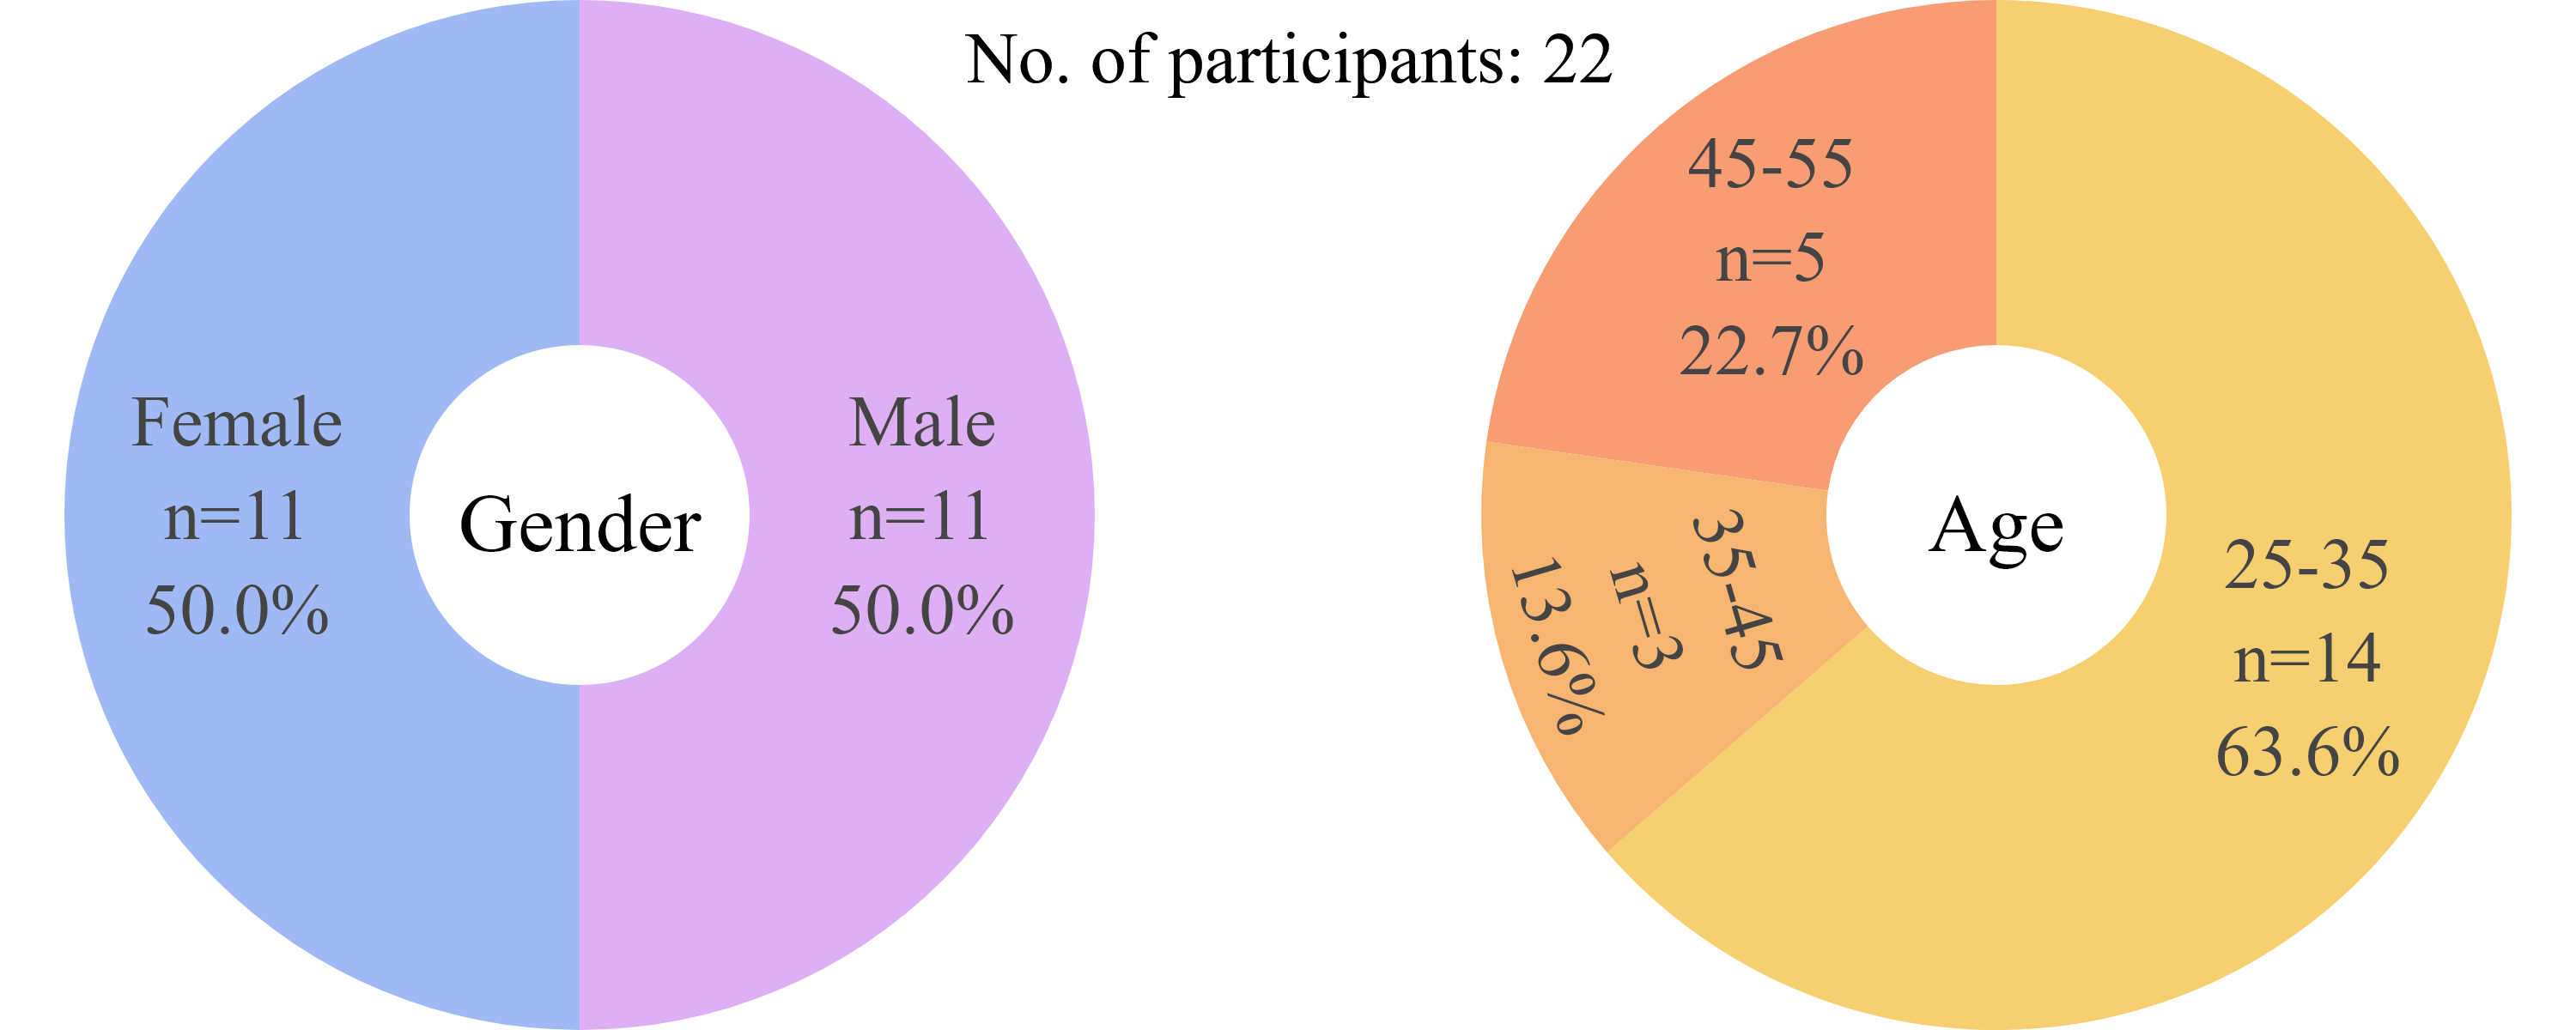
\includegraphics[width=\linewidth]{../demographics_hu}
  \caption{Demographics of the Hungarian participants.}
  \label{fig:demographics_hu}
\end{figure}

A total of 24 native Hungarian speakers filled our questionnaire, and after validating the responses (reviewing attention checks and manually checking for anomalies) 2 were rejected. Participants were recruited online using the participant recruitment platform Prolific, with screeners set for location (Hungary) and first language (Hungarian); raters were compensated for their time with a small monetary reward. In the end, the Hungarian ratings dataset had 22 participants (n=11 female, n=11 male), with ages ranges of 25-35 (n=14), 35-45 (n=3), and 45-55 (n=5). See Figure~\ref{fig:demographics_hu} for the distribution.

\subsubsection{Materials}

The Hungarian survey contained 44 items and 6 attention-check items, each a commonly occurring job title in Hungary, such as: \textit{modell} `model' or \textit{katona} `soldier', in no particular order. The attention-check items were removed from the final analysis, these were \textit{pincérnő} `waitress', \textit{titkárnő} `secretary (female)', \textit{tanárnő} `teacher (female)', \textit{takarítónő} `cleaning lady', \textit{ápolónő} `nurse (female)', and \textit{házvezetőnő} `housekeeper (female)'. These words are compounds, they explicitly determine the gender of the worker by appending \textit{-nő} `woman' to the base noun. If participants paid attention, all these items should be rated `completely female' (3). Participants who rated any of these lower than 2, or rated them lower than 3 more then once were rejected.

The 6 words above have counterparts without the \textit{nő} `woman' element, i.e. \textit{pincér} `waiter', \textit{titkár} `secretary', \textit{tanár} `teacher', \textit{takarító} `cleaner', \textit{ápoló} `nurse', and \textit{házvezető} `housekeeper', all included in our survey. These words are unmarked for gender, but they do not explicitly refer to men. The perceived gender bias of these occupations -- if any -- is due to social factors, not grammatical ones.

\hl{Maybe some of this below should go to introduction...:}

On the surface level, the unmarked form is the base noun, and the feminine-marked form is created by appending \textit{-nő} `woman' to it, which is a regular way of creating female occupational titles in Hungarian. However, in reality this does not equal to a male-female pair, as the unmarked form is not necessarily ``masculine''. We can observe 3 types in the pragmatic usage of occupational nouns when it comes to the unmarked--marked pairing and its implications for the gendering of the unmarked nouns.

1) \textbf{Both forms are common.} Frequently occuring word-pairs in Hungarian would be for example \textit{énekes} `singer' -- \textit{énekesnő} `female singer' (not in our dataset). In cases where both versions are well established -- i.e., both occur with a relatively high frequency in a balanced corpus -- the unmarked word seems to carry some male bias, as the frequent use of a feminine form indicates a need and/or custom for differentiation. We wanted to test if raters perceived this bias or not. In this example, the absolute and relative frequencies (occurrance per a million words) of the two lemmatized nouns in the Hungarian National Corpus (HNC) are 1441/9,4001 for \textit{énekes} and 748/4,8795 for \textit{énekesnő} \citep{varadi_2002_hungarian, oravecz_2014_hungarian}; the frequency difference here is roughly half (51.9\%).

The stark deviations in frequencies for marked-unmarked word pairs such as the above are not an indicator for a strong gender bias -- we can assume that both men and women singers would be equally represented in the Hungarian corpus -- but reflect that in general, the unmarked forms are used for either males or females when talking about one's occupation. The female-marked forms are used when there is an explicit intention to specify the gender of the individual, when it is otherwise not known from context (or proper names).\footnote{For example, the sentence \textit{Anyukám tanár.} `My mom is a teacher.' uses the unmarked form, firstly because we want to communicate her job, and secondly because it is obvious from the subject (mother) that she is a woman.}

2) \textbf{Only unmarked form is common.} However, there are many cases where the unmarked form is the only one generally used for both genders. Take for example \textit{ügyész} `prosecutor' (8451/55,1287) vs. \textit{ügyésznő} `female prosecutor' (56/0,3653), or \textit{fodrász} `hairdresser' (944/6,1580) vs. \textit{fodrásznő} `female hairdresser' (35/0,2283); the deviations in frequency here are over multiple orders of magnitude. In these cases, the unmarked form is the default word to describe anyone practicing the occupation, and appending \textit{'-nő} `woman' to it -- although possible -- would render it unusual, and a bit awkward; but still not as uncanny/forced as Modern English \textit{singress} would be.\footnote{Although English had a form \textit{singeress}, from Middle English \textit{syngeresse}, it is now obsolete.}

% Mention vocativus, and ügyvédnő, doktornő, tanárnő cucc... colloquial, contract would not have this! Megsy=lt's, tan'r[, tan'r ]r

3) \textbf{Marked form is common.} Furthermore, there are cases, where the female-marked version ending in \textit{-nő} is so ubiquitous, that it is the unmarked version that will sound a bit unusual, such as \textit{házvezető} `housekeeper' (10/0.0652) vs. \textit{házvezetőnő} `female housekeeper' (92/0,6001), or, to a small extent \textit{takarító} `cleaner' (169/1.1024) vs. \textit{takarítónő} `female cleaner' (392/2,5571). In short, we are interested in these unmarked words and how people perceive them.

The full list of 44 items is as follows: \textit{modell}, \textit{katona} `soldier', \textit{kórboncnok} `pathologist', \textit{vezérigazgató} `CEO', \textit{menedzser}, `manager' \textit{nővér}, `nurse' \textit{szakács} `chef', \textit{felszolgáló} `server', \textit{könyvelő} `accountant', \textit{professzor} `professor', \textit{építész} `architect', \textit{tudós} `scientist', \textit{ápoló} `nurse', \textit{pénztáros} `cashier', \textit{bíró} `judge', \textit{munkás} `worker', \textit{vízimentő} `lifeguard', \textit{jegyárus} `ticket seller', \textit{tűzoltó} `firefighter', \textit{mérnök} `engineer', \textit{rendező} `director', \textit{takarító} `cleaner', \textit{HR-es} `HR specialist', \textit{házvezető} `housekeeper', \textit{légiutas-kísérő} `flight attendant', \textit{pincér} `waiter', \textit{orvos} `doctor', \textit{fodrász} `hairdresser', \textit{földműves} `farmer', \textit{gondozó} `caregiver', \textit{bolti eladó} `shop assistant', \textit{kertész} `gardener', \textit{titkár} `secretary', \textit{PR munkatárs} `PR officer', \textit{dietetikus} `dietitian', \textit{tanár} `teacher', \textit{rendőr} `police officer', \textit{pilóta} `pilot', \textit{recepciós} `receptionist', \textit{biztonsági őr} `security guard', \textit{ügyész} `prosecutor', \textit{kozmetikus} `beautician', \textit{programozó} `programmer', \textit{diák} `student'.

We have included \textit{diák} `student' out of curiosity. Although being a student is not a job per se, but it is beyond doubt the only truly gender-neutral ``occupation'' there is, since it is mandatory for every child to go to school (both in Hungary and in China). We wanted to see if there would be would be any bias regarding this word, especially that Hungarian has a female-marked form for it -- \textit{diáklány} `girl student', appending \textit{-lány} `girl' to the base noun -- and could be considered to belong to the 1st type with a potential male bias when considered in contrast.

\subsubsection{Procedure}

Hungarian participants were instructed to rate each word on a 7-point Likert scale, ranging from \textit{completely male} to \textit{completely female}, the ratings were then converted to numerical values from -3 to +3. The scale presented in both questionnaires followed the same logic, with 0 in the middle, hence the choices were completely male (-3); mostly male (-2); somewhat male (-1); neutral/equal (0); somewhat female (+1); mostly female (+2); completely female (+3). The exact wording of the main question of the Hungarian survey was: ``Ön szerint a foglalkozás tipikusan férfi foglalkozás, vagy tipikusan női foglalkozás?'' (Is this occupation typically a man's occupation or a woman's occupation?), cf. \ref{fig:survey_hu}.

\begin{figure}[!ht]
  \centering
  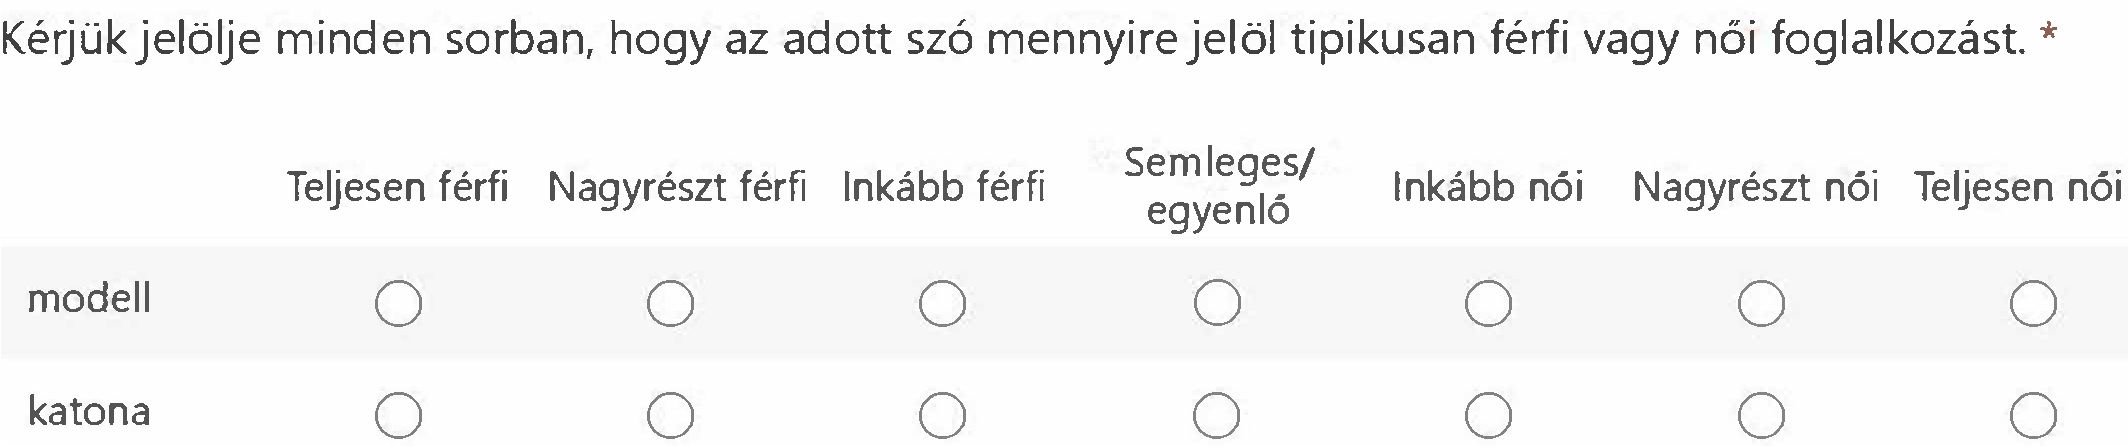
\includegraphics[width=\linewidth]{../survey_hu}
  \caption{A sample of the the Hungarian survey layout.}
  \label{fig:survey_hu}
\end{figure}

The survey was created in Microsoft Forms, and after a brief welcome message and instructions the words were presented in a simple list format, each word with a corresponding rating scale next to it, with no context. Time limit was not set, but the survey was designed to take around 5 minutes, and participants took 4 minutes 25 seconds on average to finish. 

\subsection{Chinese survey}

\subsubsection{Participants}

\begin{figure}[!ht]
  \centering
  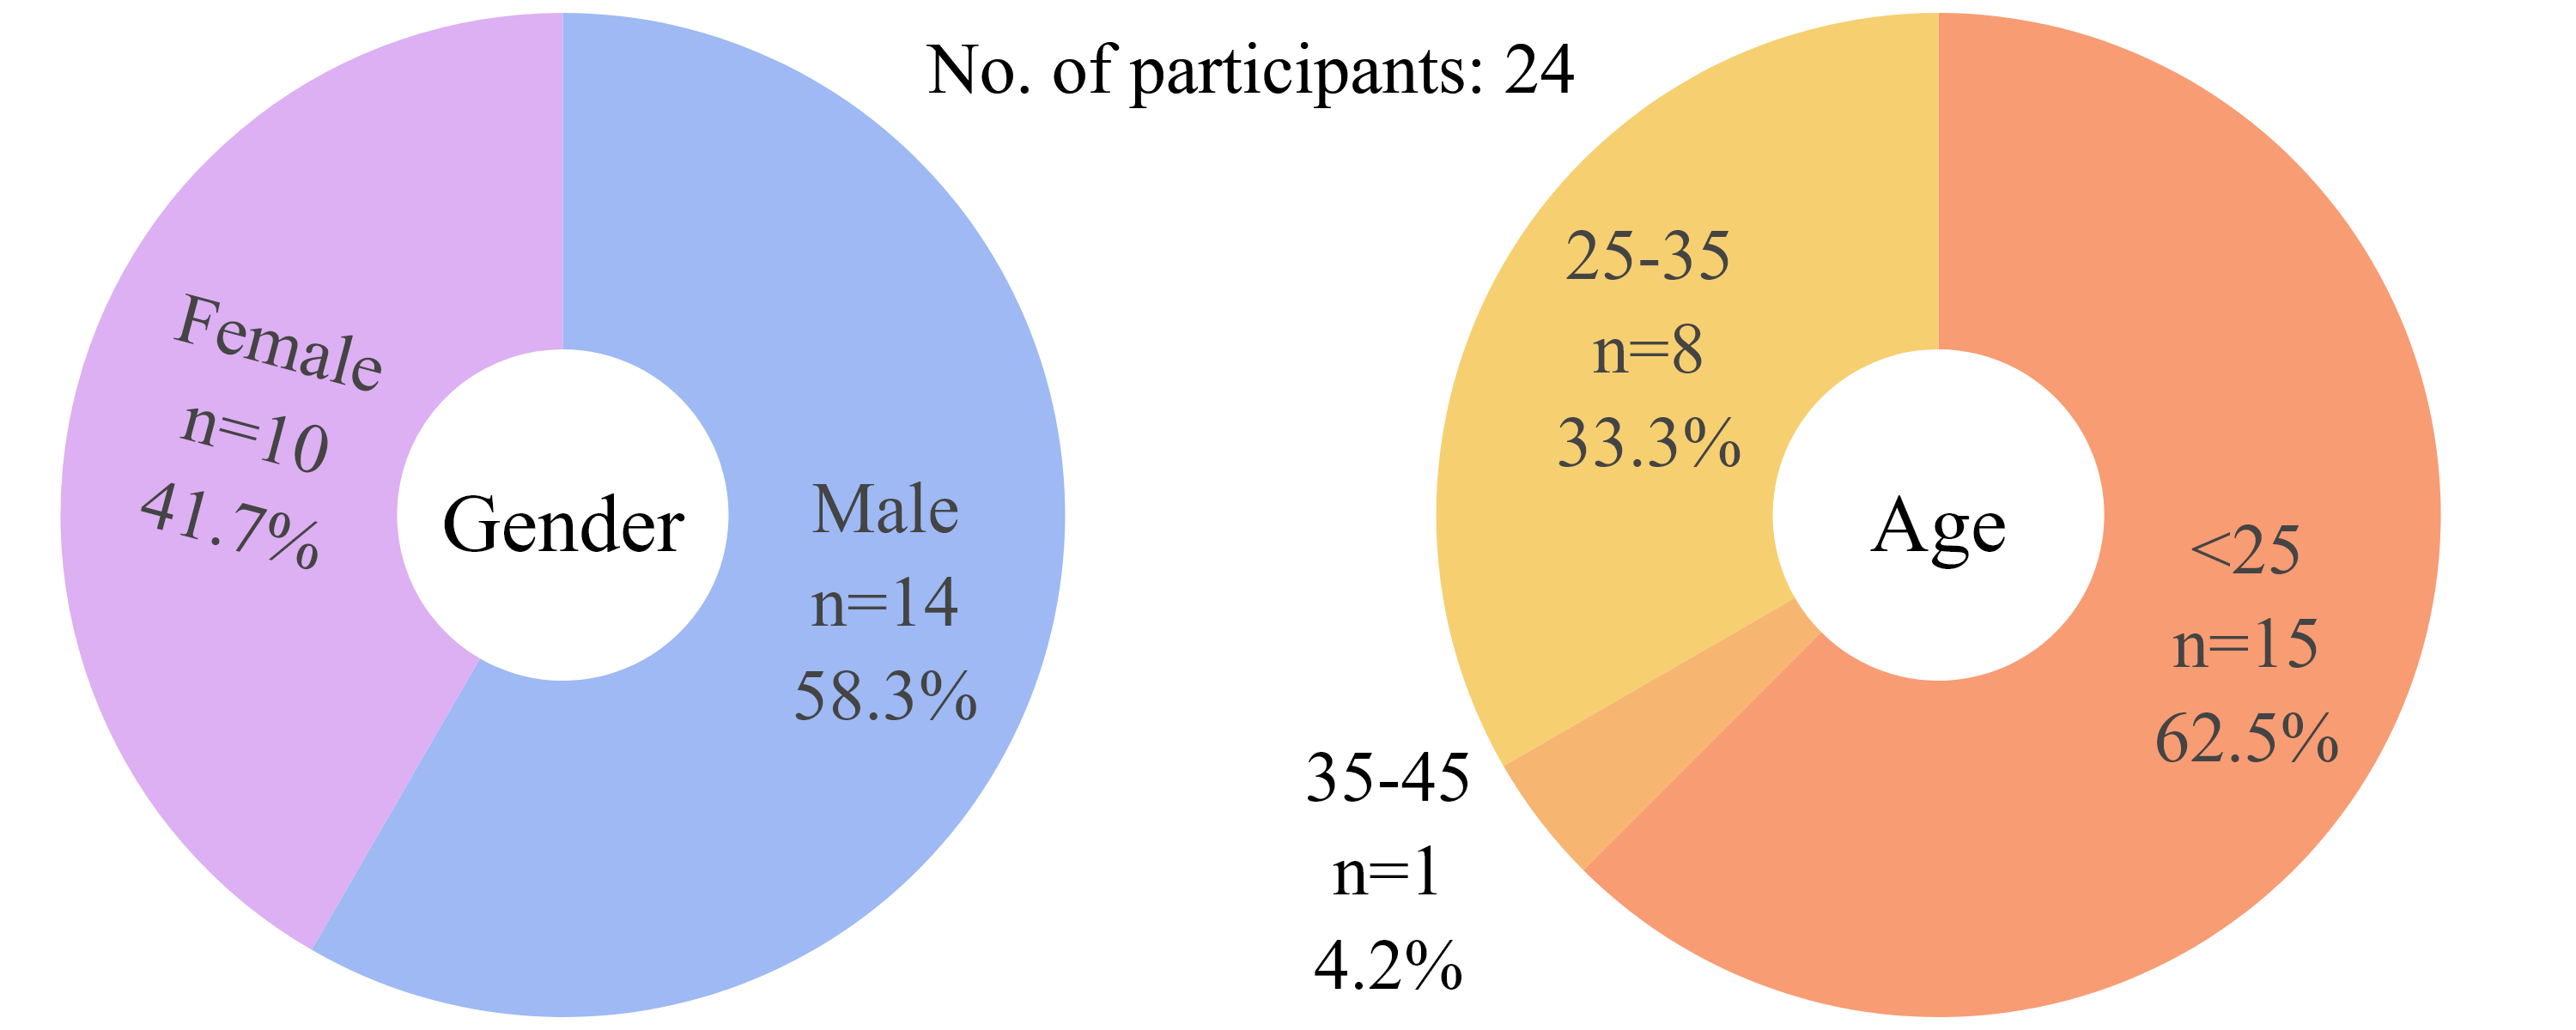
\includegraphics[width=\linewidth]{../demographics_zh}
  \caption{Demographics of the Chinese participants.}
  \label{fig:demographics_zh}
\end{figure}

The Chinese survey was completed by 30 native Mandarin Chinese speakers, 6 of which were rejected after failing attention checks. 

\hl{Wenhui: Please describe the platform used to recruit participants/how it was distributed:}

Participants were recruited from \hl{vertical} communities on WeChat in China.  They were required to have been born and raised in mainland China, with Mandarin as their primary language and the primary language spoken at home. Additionally, they must have resided in China continuously for the past five years.  This screening mechanism facilitated a prolonged social and cultural immersion experience.

Participants were paid a small fee for completing the questionnaire. The 24 accepted participants (n=14 male, n=10 female) were mostly university students, aged <25 (n=15), 25-35 (n=8), or 35-45 (n=1). See Figure~\ref{fig:demographics_zh} for the distribution.

\subsubsection{Materials}

The Chinese survey, too, contained 44 items of commonly occurring job titles in Mandarin Chinese (Simplified), with 6 attention checks, to ensure participant engagement and data quality, also in randomized order. The attention checks were \zh{妈妈} `mother', \zh{爸爸} `father', \zh{女作家} `female writer', \zh{男作家} `male writer', \zh{女画家} `female painter', \zh{男画家} `male painter'. These words are inherently feminine or masculine in meaning, or explicitly determine gender by prepending \zh{女} `woman' and \zh{男} `man', helping to filter out inattentive responses. Participants who failed to rate these with the highest scores of either \textit{completely male} or \textit{completely female} were rejected.

Here is the full list of Chinese items: \zh{警察} `police', \zh{秘书} `secretary', \zh{教授} `professor', \zh{护士} `nurse', \zh{高管} `manager', \zh{教师} `teacher', \zh{前台} `receptionist', \zh{工人} `worker', \zh{幼师} `kindergarten teacher', \zh{模特} `model', \zh{护工} `caregiver', \zh{保姆} `nanny', \zh{会计} `accountant', \zh{工程师} `engineer', \zh{保洁} `cleaner', \zh{法官} `judge', \zh{导购员} `shop assistant', \zh{美容师} `beautician', \zh{服务员} `waiter', \zh{乘务员} `flight attendant'\footnote{\hl{Also the attendant/crew on high-speed trains.}}, \zh{理发师} `hairdresser', \zh{空服员} `flight attendant'\footnote{\hl{Less frequent word; only on airplane.}}, \zh{售票员} `ticket seller', \zh{厨师} `chef', \zh{营养师} `nutritionist', \zh{家政员} `housekeeper', \zh{收银员} `cashier', \zh{医生} `doctor', \zh{法医} `pathologist', \zh{程序员} `programmer', \zh{保安} `security guard', \zh{导演} `director', \zh{军人} `soldier', \zh{董事长} `CEO', \zh{农民} `farmer', \zh{学生} `student', \zh{园丁} `gardener', \zh{飞行员} `pilot', \zh{人事} `HR personnel', \zh{消防员} `firefighter', \zh{科学家} `scientist', \zh{检察官} `prosecutor', \zh{救生员} `lifeguard', \zh{建筑师} `architect'.


\subsubsection{Procedure}

Chinese participants, too, were instructed to rate each word on a 7-point Likert scale, ranging from \textit{completely male} to \textit{completely female} with \textit{neutral/equal} in the middle, and the ratings were then converted to numerical values as explained above. The exact wording of the questions in the Chinese survey was: ``\zh{对于\hspace{0pt}\texttt{occupation}\hspace{0pt}这个职业,\hspace{0pt}您\hspace{0pt}认为\hspace{0pt}通常\hspace{0pt}担\hspace{0pt}任该职业\hspace{0pt}的男女\hspace{0pt}性别\hspace{0pt}比例\hspace{0pt}是\hspace{0pt}多少?}'' (What do you think is the ratio of men to women in \texttt{occupation}?). The survey was created in Microsoft Forms with essentially identical instructions, participants saw each word highlighted in the question above, with no other context, and were presented with the scale directly below.

\begin{figure}[!ht]
  \centering
  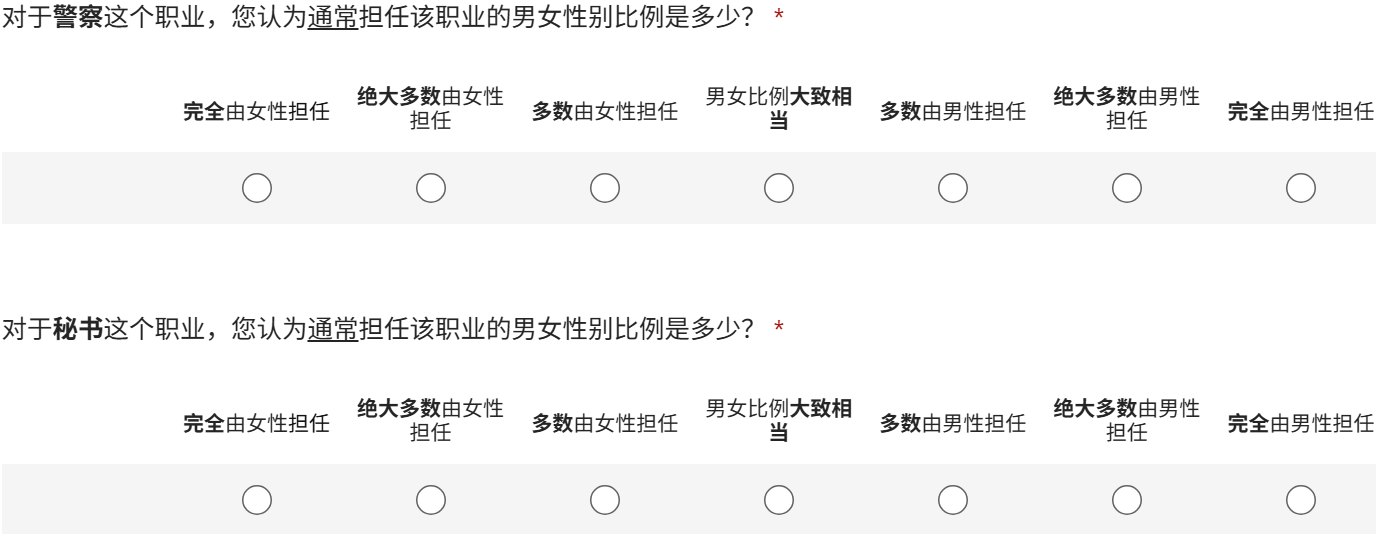
\includegraphics[width=\linewidth]{../survey_zh}
  \caption{A sample of the the Chinese survey layout.}
  \label{fig:survey_zh}
\end{figure}

\subsection{Methods}

For analyzing the data, we used the \texttt{scipy} library in Python, and performed one-sample \textit{t}-tests to determine the significance of differences in the mean ratings of occupations, and independent sample (two-sample) \textit{t}-tests to analyze the differences between different groups, such as the ratings of male and female raters and the differences between the ratings of Hungarian and Chinese raters for the same occupations. The significance level was set to $p < 0.05$, and marginally significant items (0.05 < $p < 0.1$) were also highlighted.


\section{Results \& Analysis}\label{sec:results}

For both languages, the majority of occupations were rated with a significant gender bias. In Hungarian, 36 out of 44 occupations showed significant bias, and in Chinese, 39 out of 40 were biased. This in itself is not surprising\hl{...}

\subsection{Hungarian}

\begin{figure*}[!ht]
  \centering
  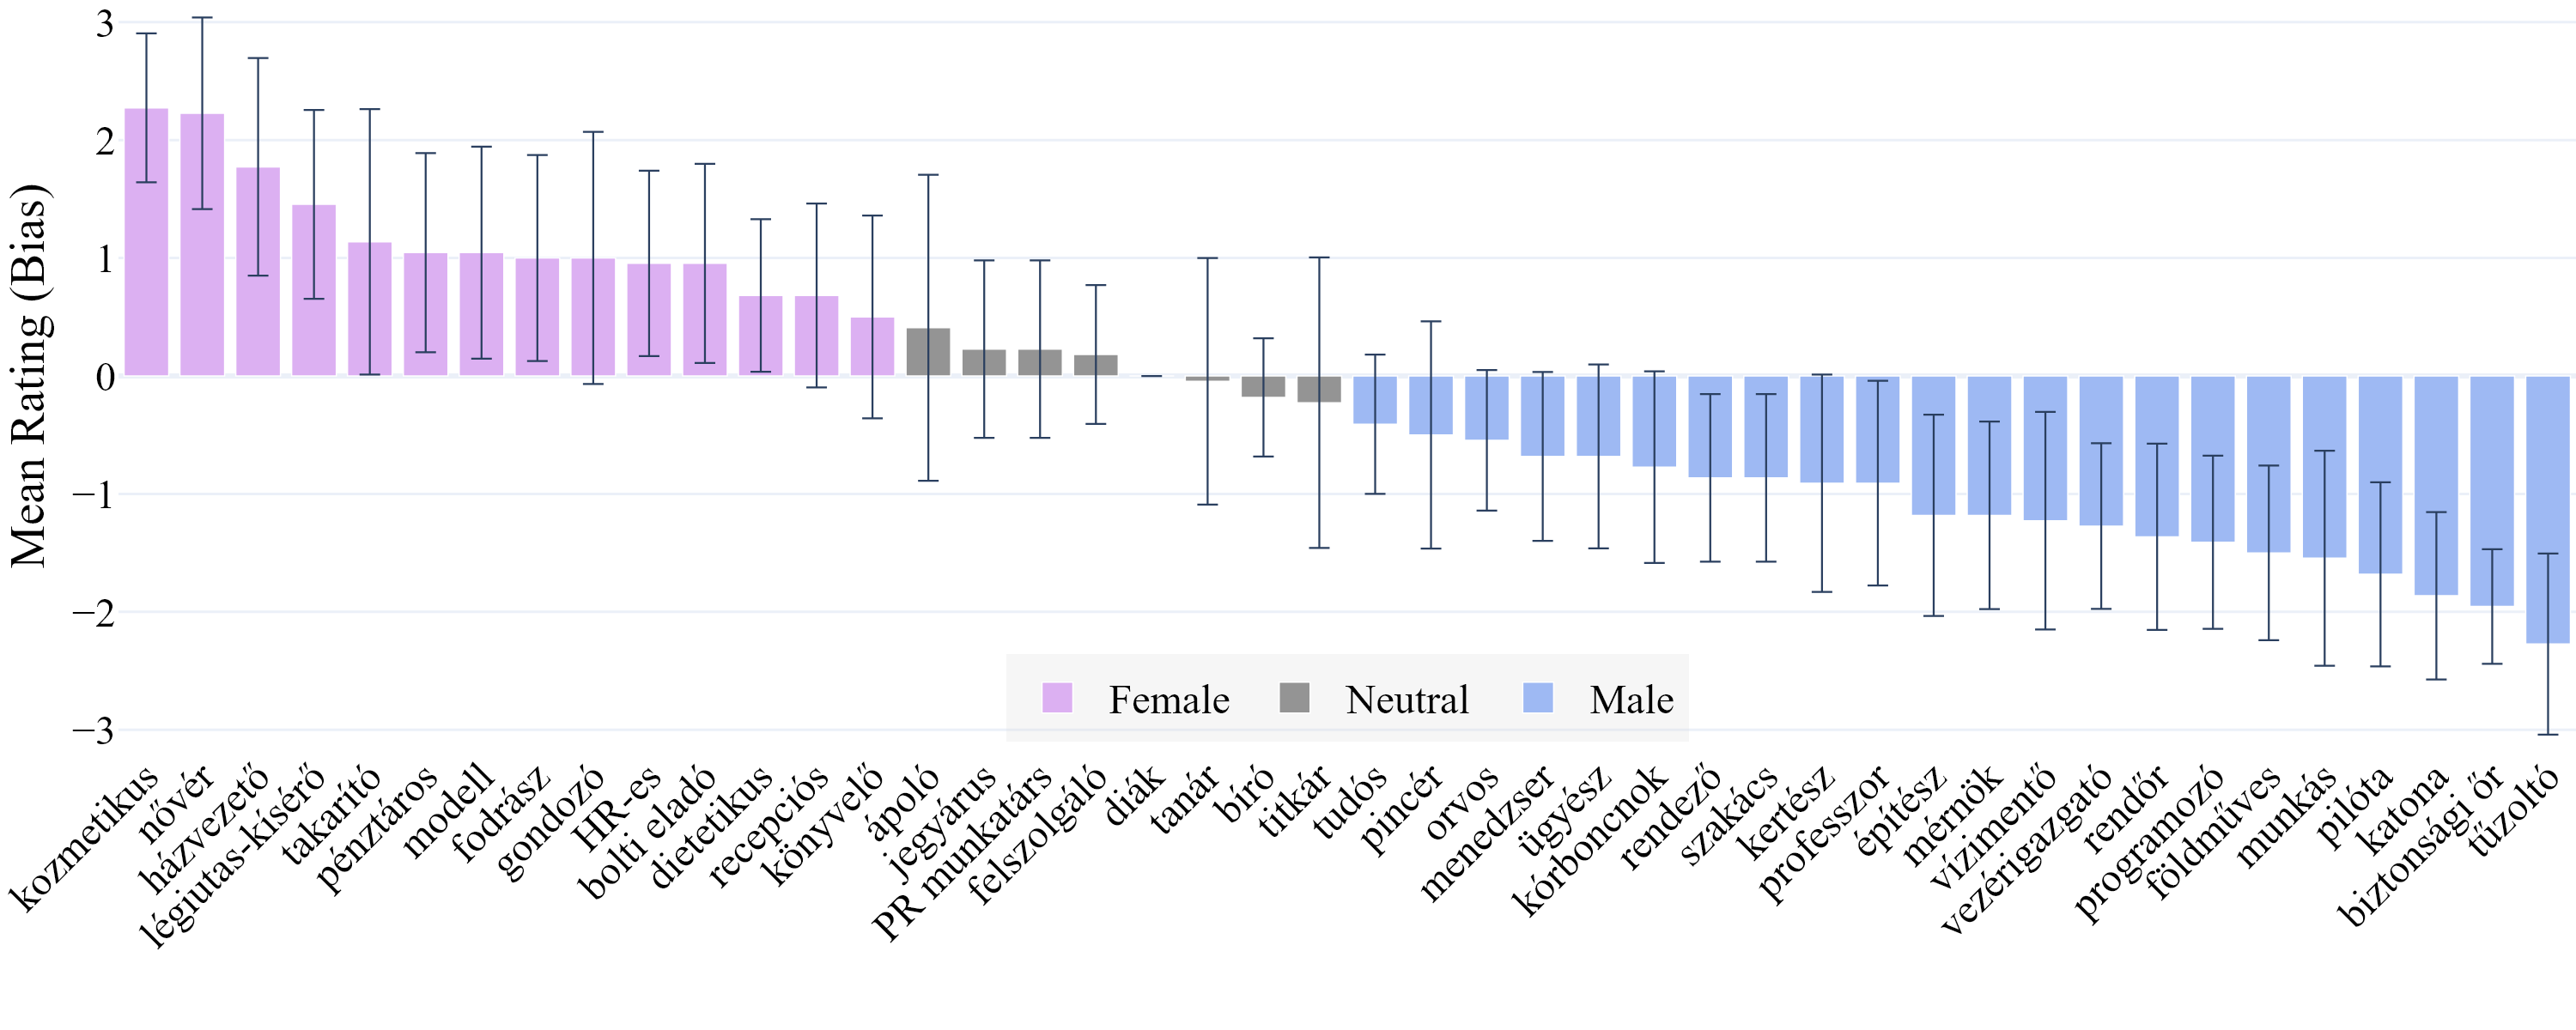
\includegraphics[width=\linewidth]{../occupations_hu}
  \caption{Mean ratings of occupational titles in Hungarian with standard deviations, significant gender bias highlighted -- \href{https://htmlpreview.github.io/?https://https://anonymous.4open.science/r/occupational-bias-paclic39/occupations_hu.html}{explore the interactive plot}.}
  \label{fig:occupations_hu}
\end{figure*}

\begin{figure*}[tbp]
  \centering
  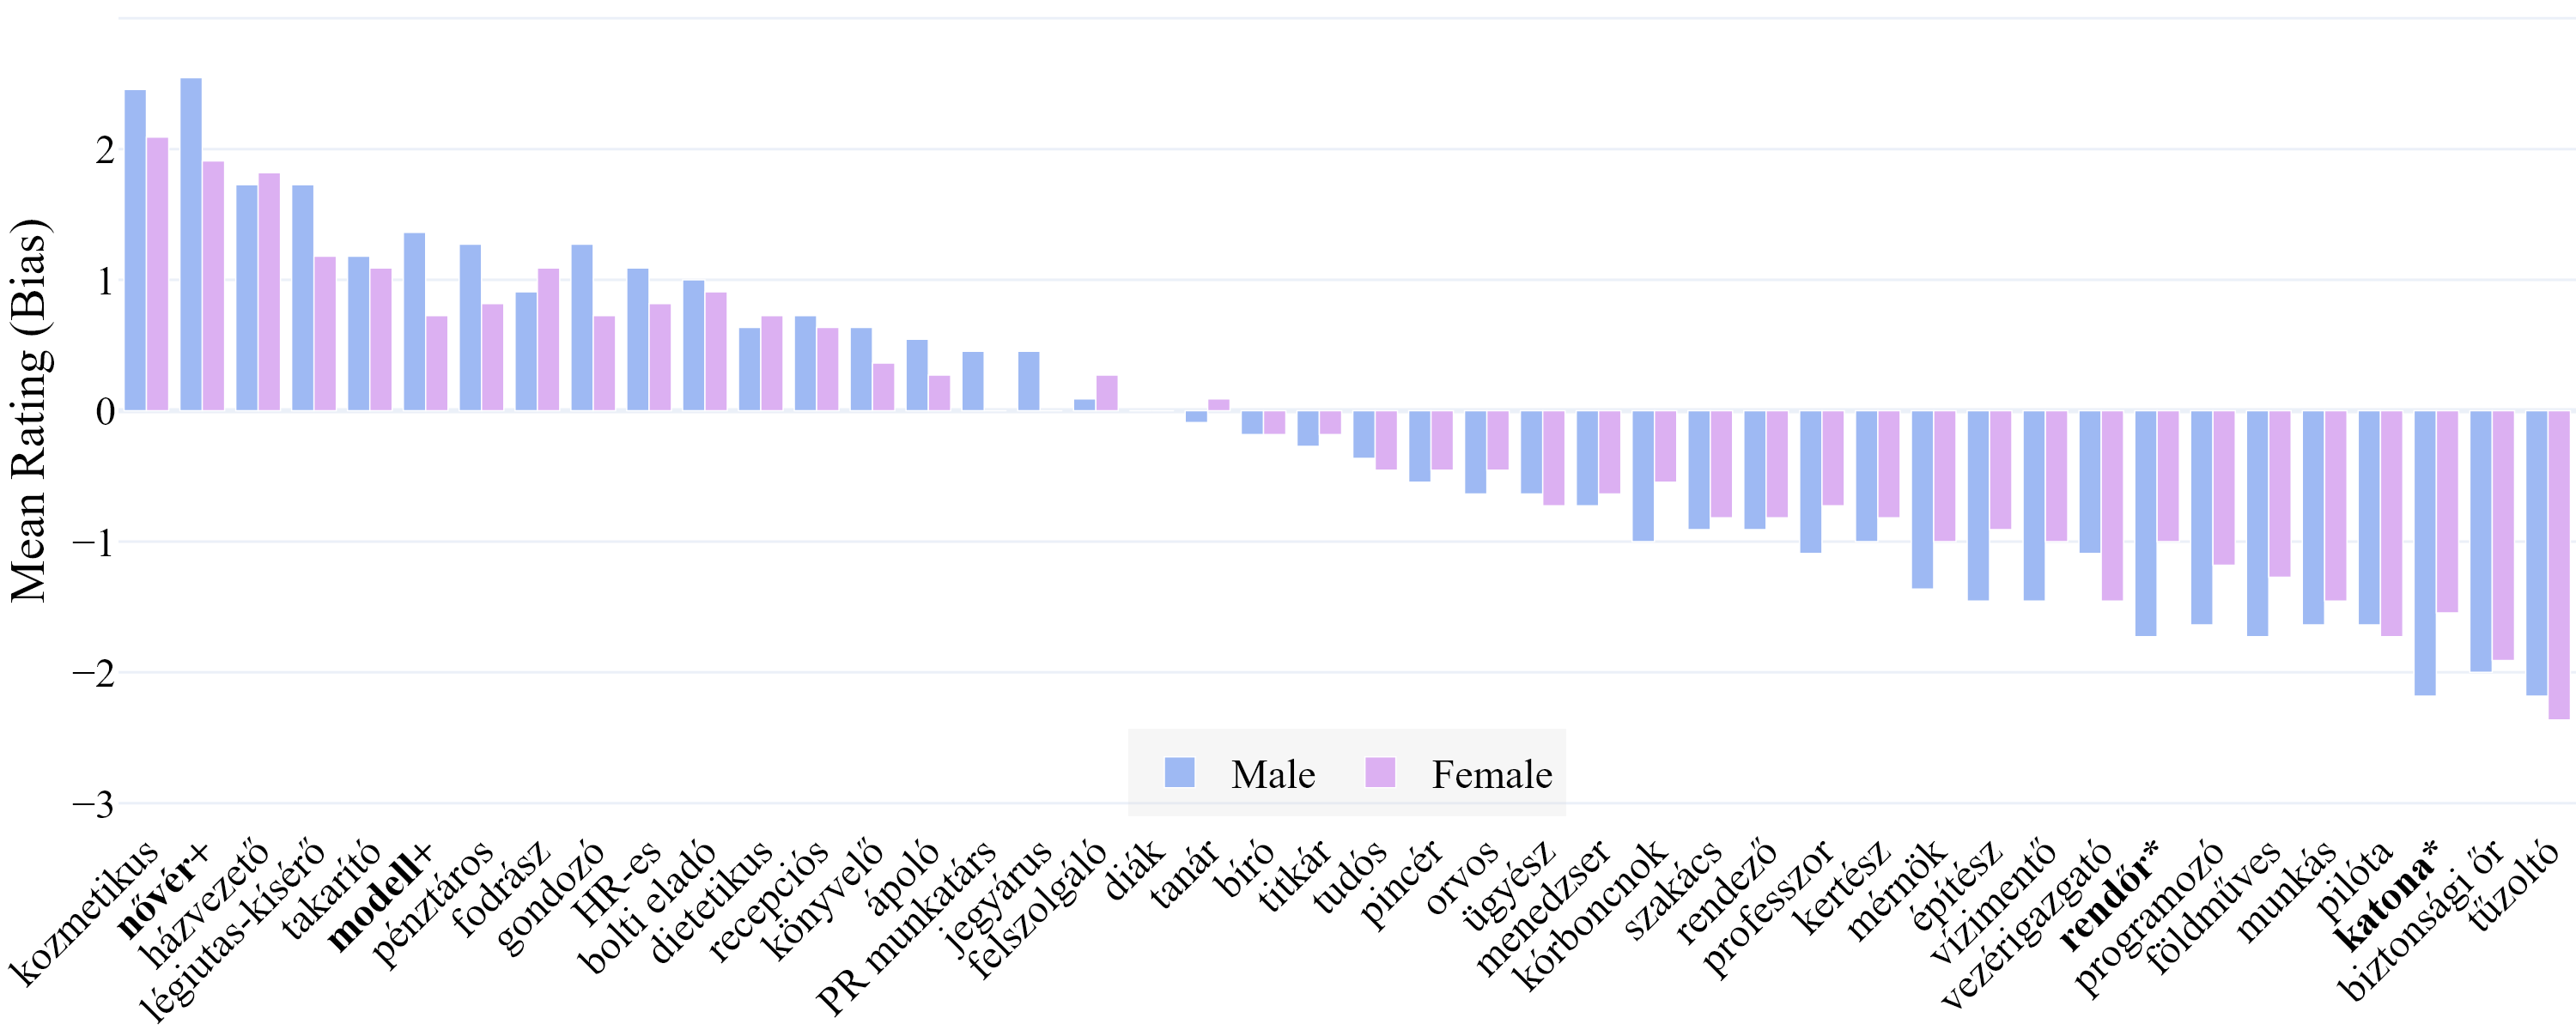
\includegraphics[width=\linewidth]{../occupations_hu_gender}
  \caption{Mean ratings of occupational titles in Hungarian by gender, significant differences highlighted (significant*, and marginally significant+ in \textbf{bold}) -- \href{https://htmlpreview.github.io/?https://github.com/partigabor/occupational-bias/blob/main/occupations_hu_gender.html}{explore the interactive plot}.}
  \label{fig:occupations_hu_gender}
\end{figure*}


The Hungarian data was first analyzed using a one-sample \textit{t}-test to determine which of the occupations showed a significant bias, measured against 0 (neutral/equal). The results showed that the majority of occupational titles -- 36 out of 44 -- were rated with a significant gender bias, with 14 showing female, and 22 showing male bias. See Figure \ref{fig:occupations_hu} for a visualization of the mean ratings, with the gender biases highlighted.


\begin{figure*}[!ht]
  \centering
  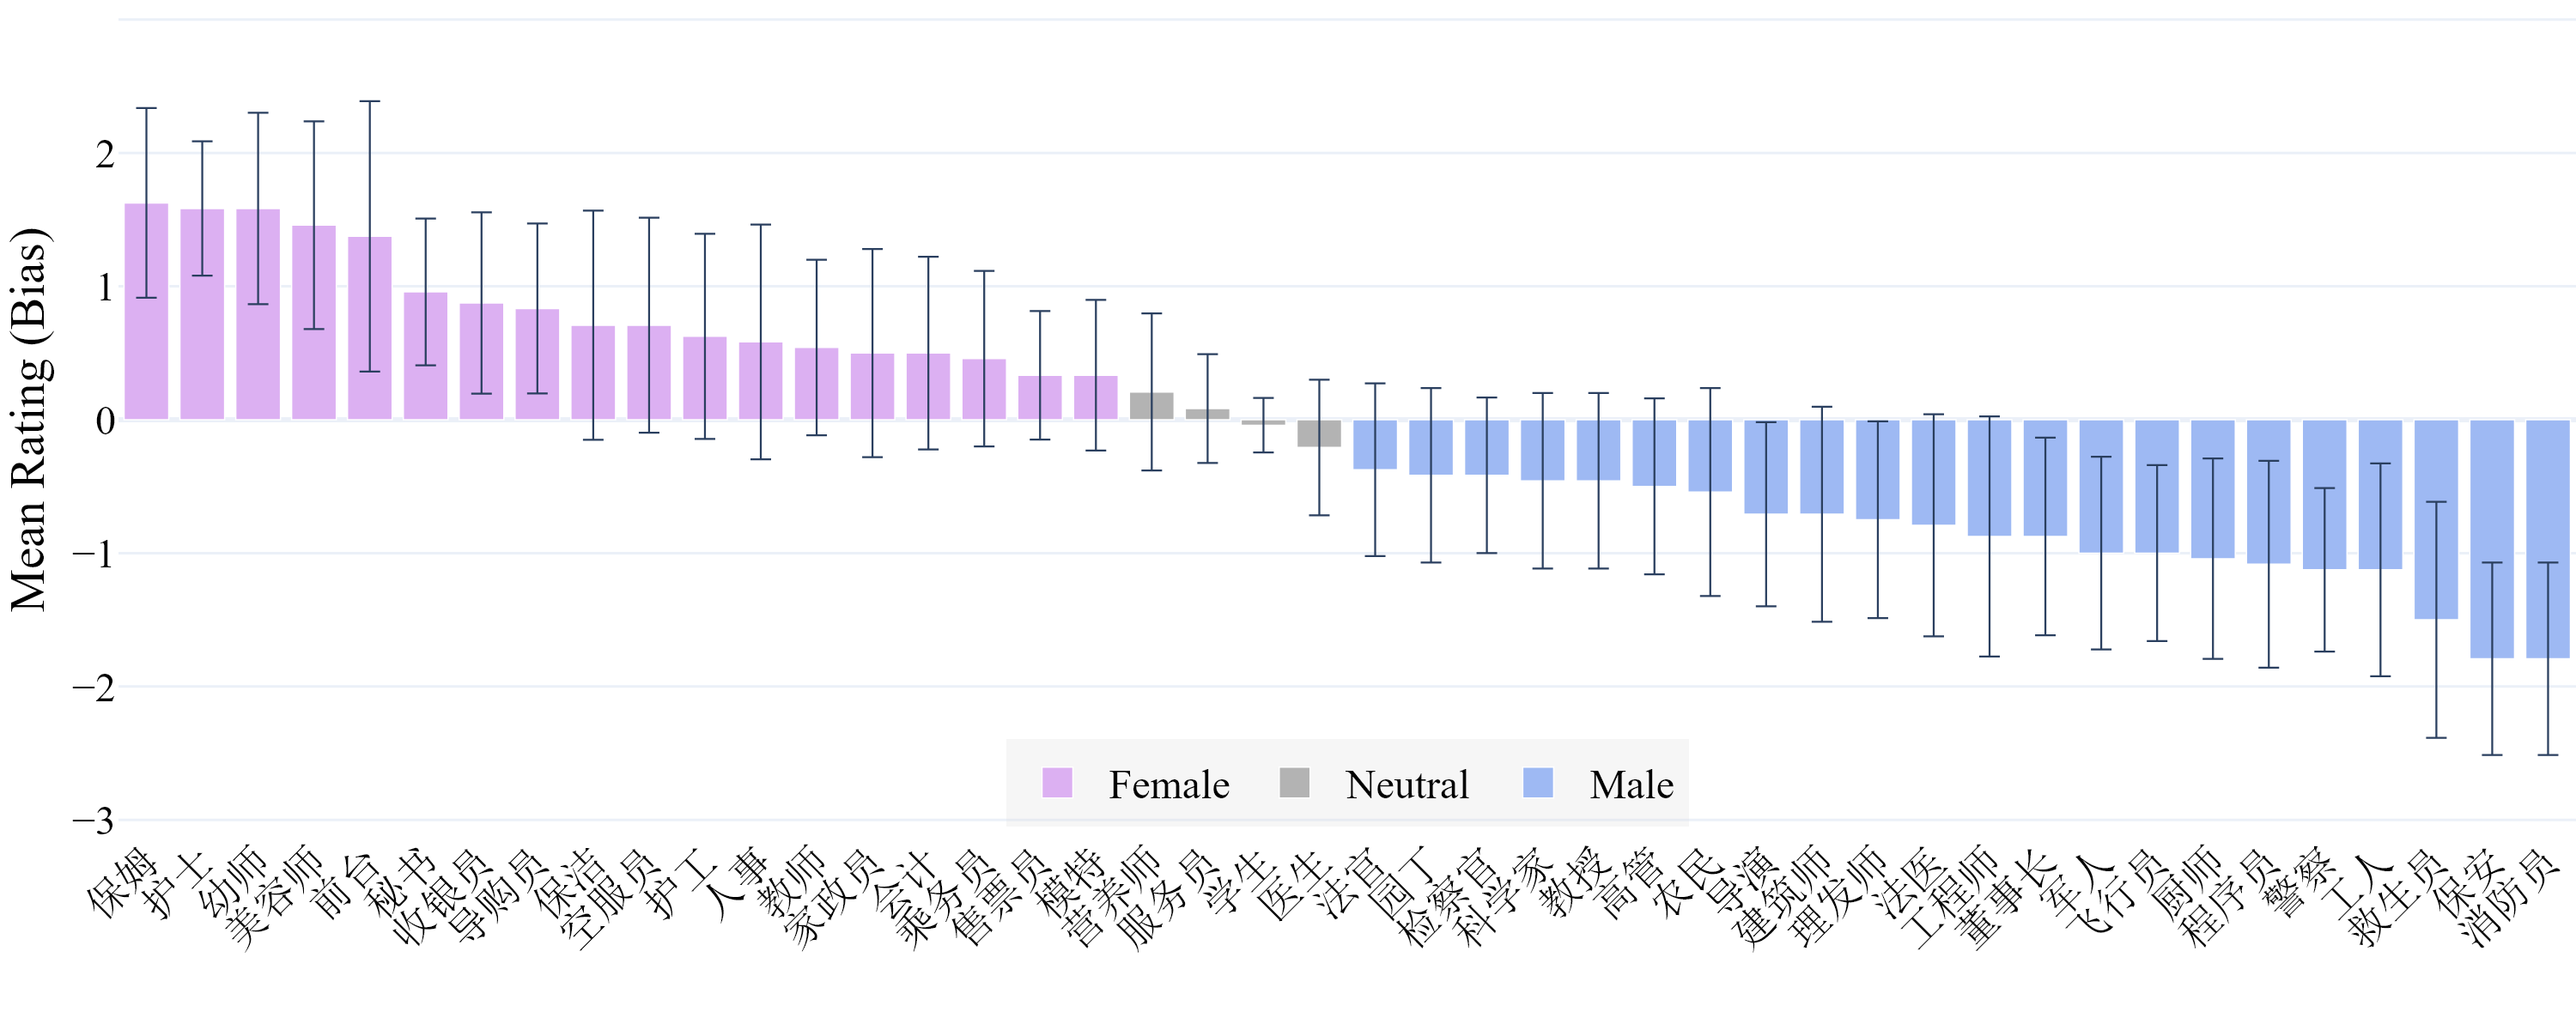
\includegraphics[width=\linewidth]{../occupations_zh}
  \caption{Mean ratings of occupational titles in Chinese with standard deviations, significant differences highlighted -- \href{https://htmlpreview.github.io/?https://github.com/partigabor/occupational-bias/blob/main/occupations_zh.html}{explore the interactive plot}.}
  \label{fig:occupations_zh}
\end{figure*}

\begin{figure*}[tbp]
  \centering
  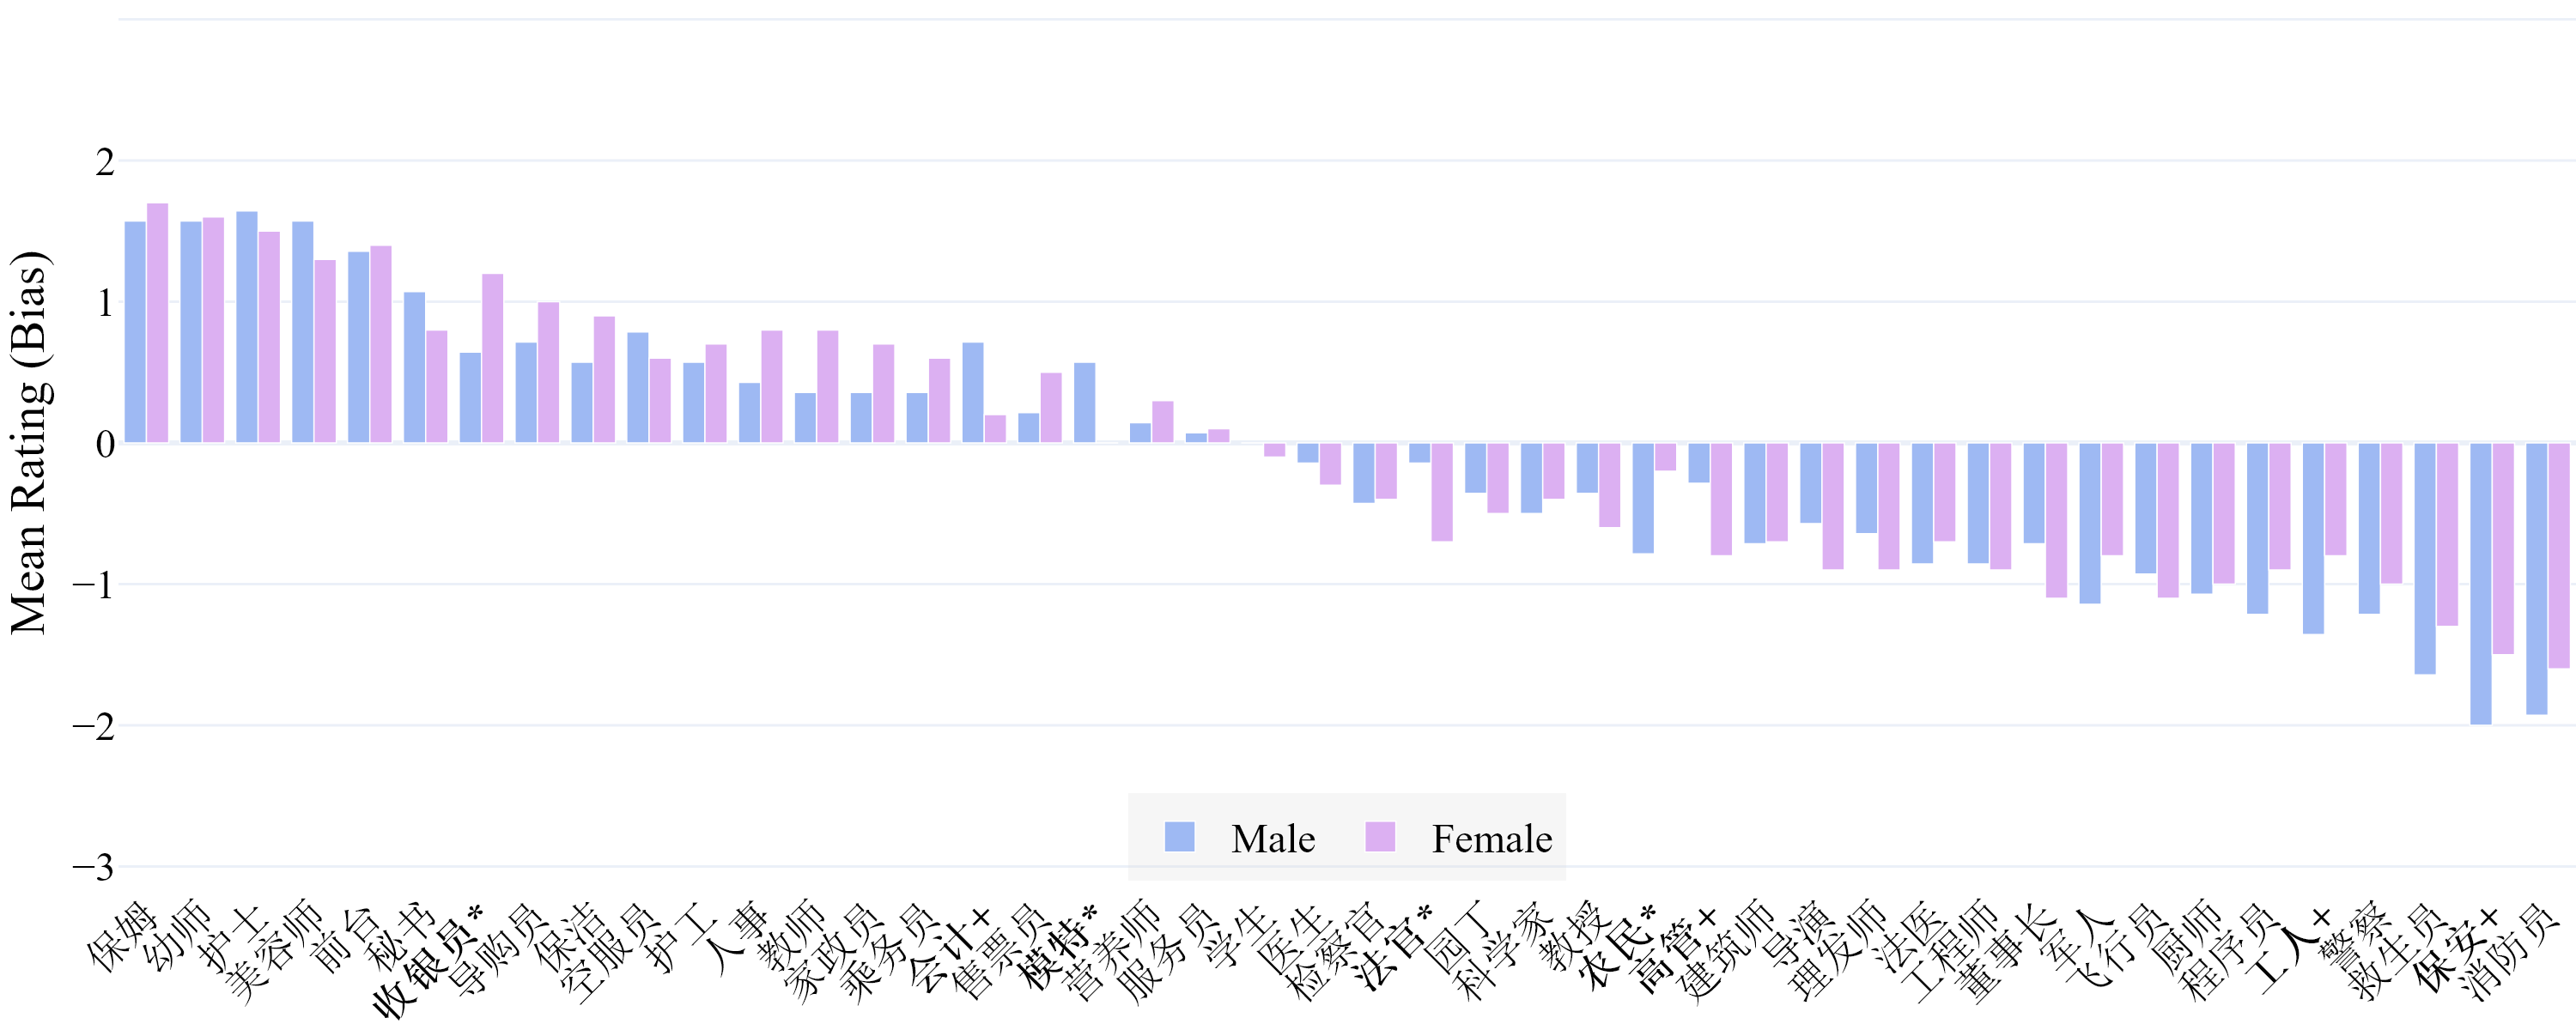
\includegraphics[width=\linewidth]{../occupations_zh_gender}
  \caption{Mean ratings of occupational titles in Chinese by gender, significant differences highlighted (significant*, and marginally significant+ in \textbf{bold}) -- \href{https://htmlpreview.github.io/?https://github.com/partigabor/occupational-bias/blob/main/occupations_zh_gender.html}{explore the interactive plot}.}
  \label{fig:occupations_zh_gender}
\end{figure*}

\subsubsection{Overall distribution of ratings}

In general, occupations were rated according to expectations, following societal stereotypes and realities. Words with the highest female bias were \textit{kozmetikus} `beautician' (2.27), \textit{nővér} `nurse' (2.23), \textit{házvezető} `housekeeper' (1.77), \textit{légiutas-kísérő} `flight attendant' (1.45), and \textit{takarító} `cleaner' (1.14), while words with the highest male bias included \textit{munkás} `worker' (-1.55), \textit{pilóta} `pilot' (-1.68), \textit{katona} `soldier' (-1.86), \textit{biztonsági őr} `security guard' (-1.95), and \textit{tűzoltó} `firefighter' (-2.27).

\textit{Nővér} `nurse' (2.23) -- is a bit special, as it literally means `sister' and goes back to the time when nuns were the ones taking care of the sick; hence the word carries a strong female bias that is encoded in its literal meaning. Interestingly, it was not rated as an exclusively female job, probably because male nurses are now also common. The gender-neutral word \textit{ápoló} `nurse' for the same job was also tested, and it received a neutral rating of 0.41.

The 8 job titles that came back as not significantly biased were: \textit{ápoló} `nurse' (0.41), \textit{jegyárus} `ticket seller' (0.23),\textit{PR munkatárs} `PR specialist' (0.23), \textit{felszolgáló} `server' (0.18),  \textit{diák} `student' (0), \textit{tanár} `teacher' (0), \textit{bíró} `judge' (-0.18), and \textit{titkár} `secretary' (-0.23). It is worth noting that while \textit{diák} `student' was rated 0 by everyone, \textit{tanár} `teacher' had more individual variation in the ratings, leading to a higher standard deviation.

The strongest agreement were on \textit{diák} `student' (0, std=0), \textit{biztonsági őr} `security guard' (-1.95; std=0.4857), \textit{bíró} `judge' (-0.18; std=0.5011), \textit{felszolgáló} `server' (0.18; std=0.5885), \textit{tudós} `scientist' (-0.41; std=0.5903).




\subsubsection{Intra-language gender differences in the Hungarian data}

We also ran a two-sample \textit{t}-test to compare the ratings of male and female participants for each occupation, and see if there was any discrepancies between the two groups. The only jobs that showed a significant difference was \textit{rendőr} `police officer' (male=-1.73; female=-1.00) and \textit{katona} `soldier' (m=-2.18; f=-1.55), here the male biases were much higher by male raters. Two marginally significant different items were also found in \textit{modell} `model' (m=1.36; f=0.73) and \textit{nővér} `nurse' (m=2.55; f=1.91) showing a similar trend. The results are summarized in Figure \ref{fig:occupations_hu_gender}.

Furthermore, it seems like men's ratings tended to have a greater absolute bias for both male- and female-coded jobs (see Figure \ref{fig:confusion_matrices} below).


\subsection{Chinese}

Similarly to Hungarian, we found that a majority of occupations in Chinese were also rated with significant gender bias. The results of the one-sample \textit{t}-test showed that 39 out of 44 occupations were biased. The mean ratings are shown in Figure \ref{fig:occupations_zh}.

\subsubsection{Overall distribution of ratings}

\hl{Wenhui, can you help here with explaining some of our expectations for the results?:}

The rating results largely aligned with our expectations concerning occupational gender stereotypes in Chinese society. Participants typically linked women to child-bearing, emotional labor, and service-oriented roles while associating men with high-intensity, high-risk physical labor, and order-maintaining roles.

In Chinese, the words with the highest female bias were \zh{保姆} `domestic helper' (1.63), \zh{护士} `nurse' (1.58), \zh{幼师} `kindergarten teacher' (1.58), \zh{美容师} `beautician' (1.46), and \zh{前台} `receptionist' (1.38). Words with the highest male bias were \zh{警察} `police officer' (-1.13), \zh{工人} `worker' (-1.13), \zh{救生员} `lifeguard' (-1.50), \zh{保安} `security guard' (-1.79), and \zh{消防员} `firefighter' (-1.79), which shows a relatively strong similarity to the Hungarian trends.

The 4 job titles that were not significantly biased were: \zh{营养师} `dietitian' (0.21), \zh{服务员} `waiter/server' (0.08), \zh{学生} `student' (-0.04), and \zh{医生} `doctor' (-0.21).

In Chinese too, there was strong agreement on \zh{学生} `student' (-0.04; std=0.2041) and \zh{服务员} `water/server' (0.08; std=0.4082), the remaining words in the top 5 jobs with the lowest standard deviation were \zh{售票员} `ticket seller' (0.33; std=0.4815), \zh{护士} `nurse' (1.58; std=0.5036), and \zh{医生} `doctor' (-0.21; std=0.5089).

\begin{figure*}[!ht]
  \centering
  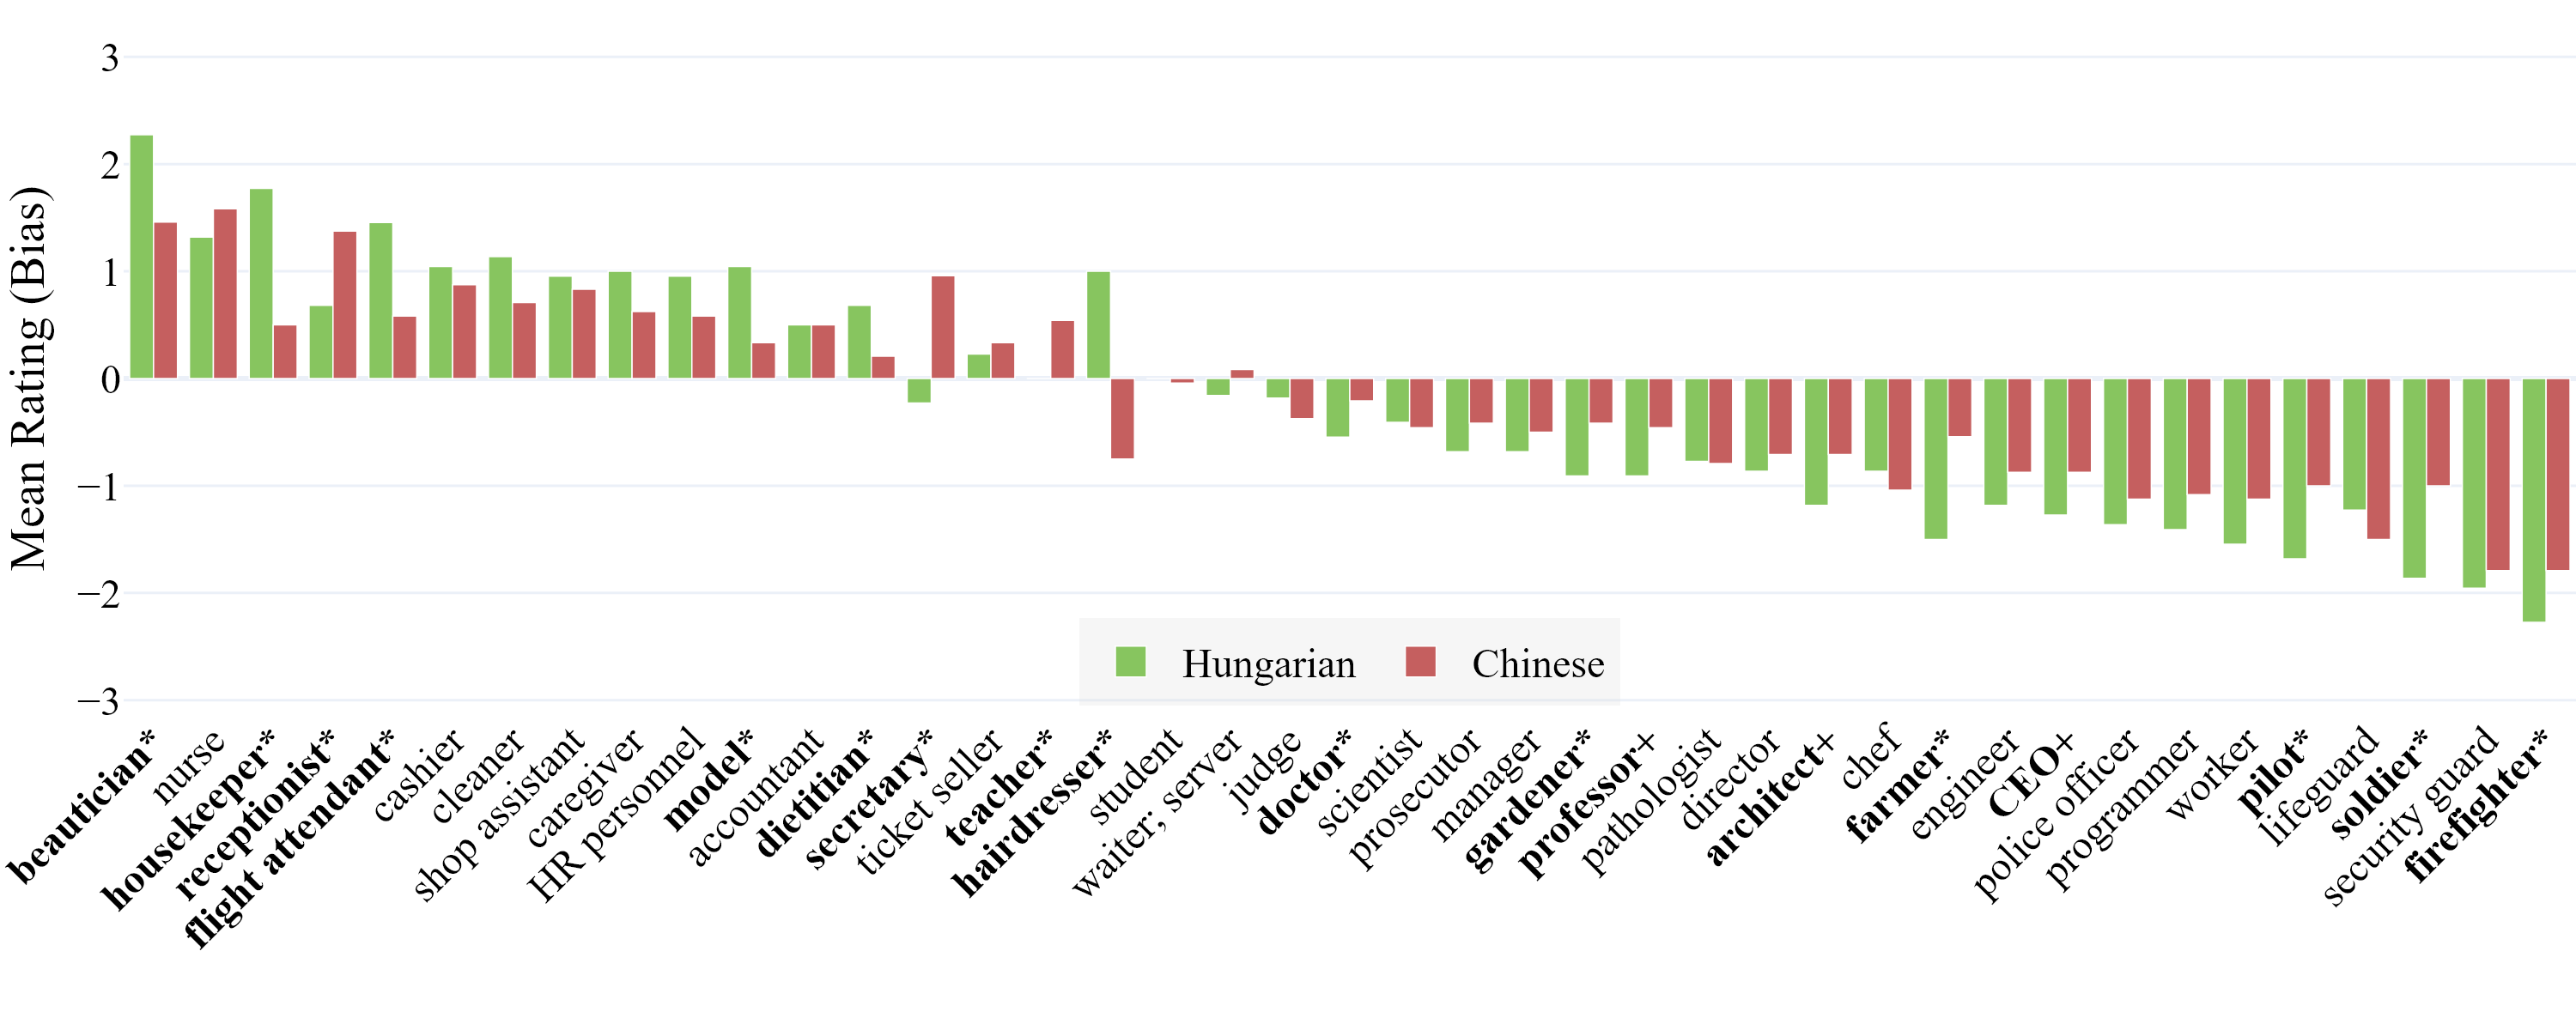
\includegraphics[width=\linewidth]{../occupations_comparison}
  \caption{Mean ratings of common occupational titles in Hungarian and Chinese (significant*, and marginally significant+ in \textbf{bold}) -- \href{https://htmlpreview.github.io/?https://github.com/partigabor/occupational-bias/blob/main/occupations_comparison.html}{explore the interactive plot}.}
  \label{fig:occupations_comparison}
\end{figure*}

\subsubsection{Intra-language gender differences in the Chinese data}

The two-sample \textit{t}-test comparing the ratings of male vs. female participants showed that there were significant differences between what people think of a typical \zh{收银员} `cashier' (m=0.64; f=1.20), \zh{模特} `model' (m=0.57; f=0), \zh{法官} `judge' (m=-0.14; f=0.70), and \zh{农民} `farmer' (m=-0.79; f=-0.20). Marginally significant differences were found for \zh{会计} `accountant' (m=0.71; f=0.20), \zh{高管} `manager' (m=-0.29; f=-0.80), \zh{工人} `worker' (m=-1.36; f=-0.80), and \zh{保安} `security guard' (m=-2.00; f=-1.50). The results can be examined in Figure \ref{fig:occupations_zh_gender}.


\subsection{Cross-linguistic comparison}

% * **Comparison with Large Language Models (LLMs)**:
%     * Briefly introduce the data from ChatGPT, Gemini, etc., as a point of comparison. You can include the *occupations_hu_llms.png* or *occupations_zh_llms.png* plot.
%     * Note how the LLMs often show even stronger biases than human participants, and their ratings align with the general trends observed in the human data. This adds a modern, impactful layer to your paper.

The wordlists of the two datasets were almost, but not exactly the same; by performing an inner join on the two lists, we could pair 42 items together according to their meanings. Then, using a two-sample \textit{t}-test, we checked if there were significant differences between the ratings in the two languages. The results are summarized in Figure \ref{fig:occupations_comparison}.

When comparing the two sets of ratings, the first noticeable trend is that in general, the two languages have similar biases for the same occupations. Shared items on the extreme ends of the scale include for example `beautician' and `nurse', as well as `firefighter' and `security guard'. Job titles that were neutral/unbiased in both datasets were `server' (\textit{felszolgáló}; \zh{服务员}), and `student' (\textit{diák}; \zh{学生}).

% Significant differences between Hungarian and Chinese ratings:
% Number of significant differences: 16
% en	hu	zh	mean_hu	mean_zh	mean_difference	t_stat	p_value
% 17	hairdresser	fodrász	理发师	1.000000	-0.750000	1.750000	7.312200	5.736294e-09
% 18	housekeeper	házvezető	家政员	1.772727	0.500000	1.272727	5.029788	1.000443e-05
% 15	flight attendant	légiutas-kísérő	乘务员	1.454545	0.458333	0.996212	4.587243	4.222435e-05
% 13	farmer	földműves	农民	-1.500000	-0.541667	-0.958333	-4.278163	1.002276e-04
% 35	soldier	katona	军人	-1.863636	-1.000000	-0.863636	-4.086543	1.837751e-04
% 32	secretary	titkár	秘书	-0.227273	0.958333	-1.185606	-4.151098	2.721353e-04
% 4	beautician	kozmetikus	美容师	2.272727	1.458333	0.814394	3.909669	3.202907e-04
% 25	pilot	pilóta	飞行员	-1.681818	-1.000000	-0.681818	-3.187231	2.735591e-03
% 22	model	modell	模特	1.045455	0.333333	0.712121	3.185239	3.047684e-03
% 30	receptionist	recepciós	前台	0.681818	1.375000	-0.693182	-2.611683	1.237726e-02
% 9	dietitian	dietetikus	营养师	0.681818	0.208333	0.473485	2.590567	1.306656e-02
% 39	waiter	pincér	服务员	-0.500000	0.083333	-0.583333	-2.631147	1.372320e-02
% 14	firefighter	tűzoltó	消防员	-2.272727	-1.791667	-0.481061	-2.186080	3.429839e-02
% 37	teacher	tanár	教师	0.000000	0.541667	-0.541667	-2.113894	4.166036e-02
% 16	gardener	kertész	园丁	-0.909091	-0.416667	-0.492424	-2.073820	4.500390e-02
% 11	doctor	orvos	医生	-0.545455	-0.208333	-0.337121	-2.054340	4.627231e-02

In terms of significant differences, we found 16 occupations that were rated differently in the two languages. These include `beautician' (Hungarian=2.27 vs. Chinese=1.46), `housekeeper' (H=1.77 vs. C=0.50), `receptionist' (H=0.68 vs. C=1.38), `flight attendant' (H=1.45 vs. C=0.46), `model' (H=1.05 vs. C=0.33), `dietitian' (H=0.68 vs. C=0.21), `'secretary' (H=-0.23 vs. C=0.96), `teacher' (H=0.00 vs. C=0.54), `hairdresser' (H=1.00 vs. C=-0.75), `waiter' (H=-0.50 vs. C=0.08), `doctor' (H=-0.55 vs. C=-0.21), `gardener' (H=-0.91 vs. C=-0.42), `farmer' (H=-1.50 vs. C=-0.54),  `pilot' (H=-1.68 vs. C=-1.00), and `soldier' (H=-1.86 vs. C=-1.00), and `firefighter' (H=-2.27 vs. C=-1.79). Marginally significant differences were found for `professor', `architect' and `CEO'. 

\hl{--- Wenhui, this is where you can try and discuss some of these significantly different words that could be interesting for readers. For example, you can help to explain that:} 

---

The occupational title `secretary' elicits significantly different gender stereotypes among Hungarian and Chinese participants, which is a noteworthy observation. Hungarian participants perceive `titkár' as a male-dominated profession (-0.23), whereas Chinese participants perceive it a predominantly female occupation (0.96). This discrepancy may arise from the interaction of lexical attributes and cultural context. In Hungarian, `titkár' denotes both senior political officials and regular administrative employees. Conversely, the Chinese Occupational Classification Dictionary (Occupational Code: 3-01-02-02) delineates a \zh{秘书} \textit{mìshū} `secretary' as an office service employee involved in clerical and meeting-related responsibilities. This definition may delay the manifestation of in societal perception and gender expectations, yet it largely corresponds with public expectations of the secretary profession. The semantic scope and societal expectations of identical occupational titles in Hungarian and Chinese illustrate how cultural background influences gender bias in vocabulary.

The gender stereotype linked to `housekeeper' is predominantly female in both cultures; however, the extent of this bias varies considerably (Chinese: 0.5 vs. Hungarian: 1.77). In the results of Chinese participants, it is pertinent to compare the terms \zh{家政员} \textit{jiāzhèngyuán} meaning `housekeeper' and \zh{保姆} \textit{baómǔ} meaning `nanny', which are analogous in meaning yet vary in register. While the term `housekeeper' (0.5) demonstrates less gender bias than the colloquial term `nanny' (1.63), it remains categorised as a female-dominated profession due to the traditional female-associated traits of household tasks and emotional management suggested by the central term \zh{家政} \textit{jiāzhèng} `housekeeping'. This domain-specific scoring disparity indicates that although the formal and informal characteristics of occupational terminology mitigate gender stereotypes, societal gender stereotypes regarding occupations may be intricately linked to the semantic implications of language. Particular terminology related to domestic or emotional labour is more prone to evoke conventional female gender bias perceptions, thus reinforcing the gendered classification of professions.

The disparities in gender perception between `farmer' and `worker' are particularly significant. Data from Chinese participants indicates that `farmer' (-0.54) demonstrates a comparatively weaker male orientation than `worker' (-1.13), whereas in Hungarian, the two are nearly identical (farmer: -1.50 vs. worker: -1.55). This discrepancy can be attributed to China’s societal and economic development trajectory. Throughout the era of collective farming in China (1950s–-1970s), the work-point accounting system and production brigades promoted women's involvement in agricultural labour, while slogans such as ``Women hold up half the sky'' (\zh{妇女能顶半边天}) enhanced the visibility of women in this sector \citep{jacka_1997_agriculture,jacka_1997_domestic}. Despite the Household Contract Responsibility System established in the 1980s reinforcing the dominance of male household heads and consequently marginalising women's land rights \citep{zhu_2009_gender}, the significance of women in agricultural production has progressively become apparent [data is needed here to show the proportion of women in the Chinese agriculture industry]. During this period, township enterprises and factories employed female labour; however, they confined women to light industrial positions through technical qualification prerequisites \citep{liu_2007_gender}. This led to a gendered labour division in which women in industry participated in unskilled roles, while men retained technical monopolies \citep{bossen_2002_chinese}. This historical process has resulted in the ongoing divergence of gender perceptions between the agricultural and industrial sectors. Despite contemporary ideals of occupational gender equality, gender stereotypes in lower-tier professions continue to demonstrate significant historical persistence.

% Bossen, L. (2002). Chinese Women and Rural Development (1st ed.). Bloomsbury Publishing. 
% Jacka, T. (1997). Domestic work. In Women’s Work in Rural China: Change and Continuity in an Era of Reform (pp. 101–119). Cambridge University Press. https://doi.org/10.1017/CBO9780511518157.007 
% Jacka, T. (1997b). Agriculture. In Women’s Work in Rural China: Change and Continuity in an Era of Reform (pp. 120–142). Cambridge University Press. https://doi.org/10.1017/CBO9780511518157.008 
% Liu, J. (2007). Gender and work in urban china: Women workers of the unlucky generation (pp. 47–49). Routledge. 
% Zhu, L. (2009). Gender Inequality in the Land Tenure System of Rural China. In Z. Deng (Ed.), China’s economy: Rural reform and agricultural development (pp. 21–36). World Scientific. https://doi.org/10.1142/9789814293327_0002 

---

--- housekeeper is not exactly the same as \zh{家政员} (housekeeper in Hungarian is equal to a maid, major tasks are cleaning and cooking. I heard that \zh{家政员} is more serious.)

--- secretary has more than one meaning (I don't know Chinese, but Hungarian yes, one is a secretary of a political party (leadership position), other is a personal assistant (subordinate).)

--- whatever else you can say about the significantly different words.

--- the top 10 most different occupations in order are: `hairdresser', `housekeeper', `flight attendant', `farmer', `soldier', `secretary', `beautician', `pilot', `model', and `receptionist'.

\dots

The most striking dissimilarity was the word for `hairdresser' (\textit{fodrász} vs. \zh{理发师}), which shows a strong female bias in Hungarian (1.00) but a definite male bias in Chinese (-0.75). We believe that this is a neat example for a cultural difference, in Hungary hairdressers are perceived to be predominantly female, while in China the profession is perceived to be more male-dominated. It is not difficult to find evidence for the latter from the press, even in English-language media.\footnote{\href{https://www.chinadailyhk.com/hk/article/603100}{https://www.chinadailyhk.com/hk/article/603100}}

\dots

\subsection{Discussion}\label{sec:discussion}

The first obvious thing to notice when looking at Figure \ref{fig:occupations_comparison} is that the overall trends in gender bias are quite similar between the two languages, despite some notable differences in specific occupations. This suggests that stereotypes are comparable and -- mostly -- consistent across developing societies.

It would be interesting not only to explore the reasons behind this difference, but to compare actual figures on the gender distribution of hairdressers in the two countries, and see if the ratings reflect reality. \hl{(Is there any available workforce statistics on gender distribution per profession?)}

--- many service jobs?

\subsection{Gender bias by language}

An interesting feature is that Hungarian raters tended to rate occupations with a stronger bias than Chinese speakers. Out of 42 shared occupations, 31 were rated with a higher bias in Hungarian, while only 10 were rated with a higher bias in Chinese (excluding the 1 item with equal value). This is a threefold difference, and warrants further exploration to fully explain.

\hl{Tie in Kaukonen et al. here}

\begin{figure}[ht]
  \centering
  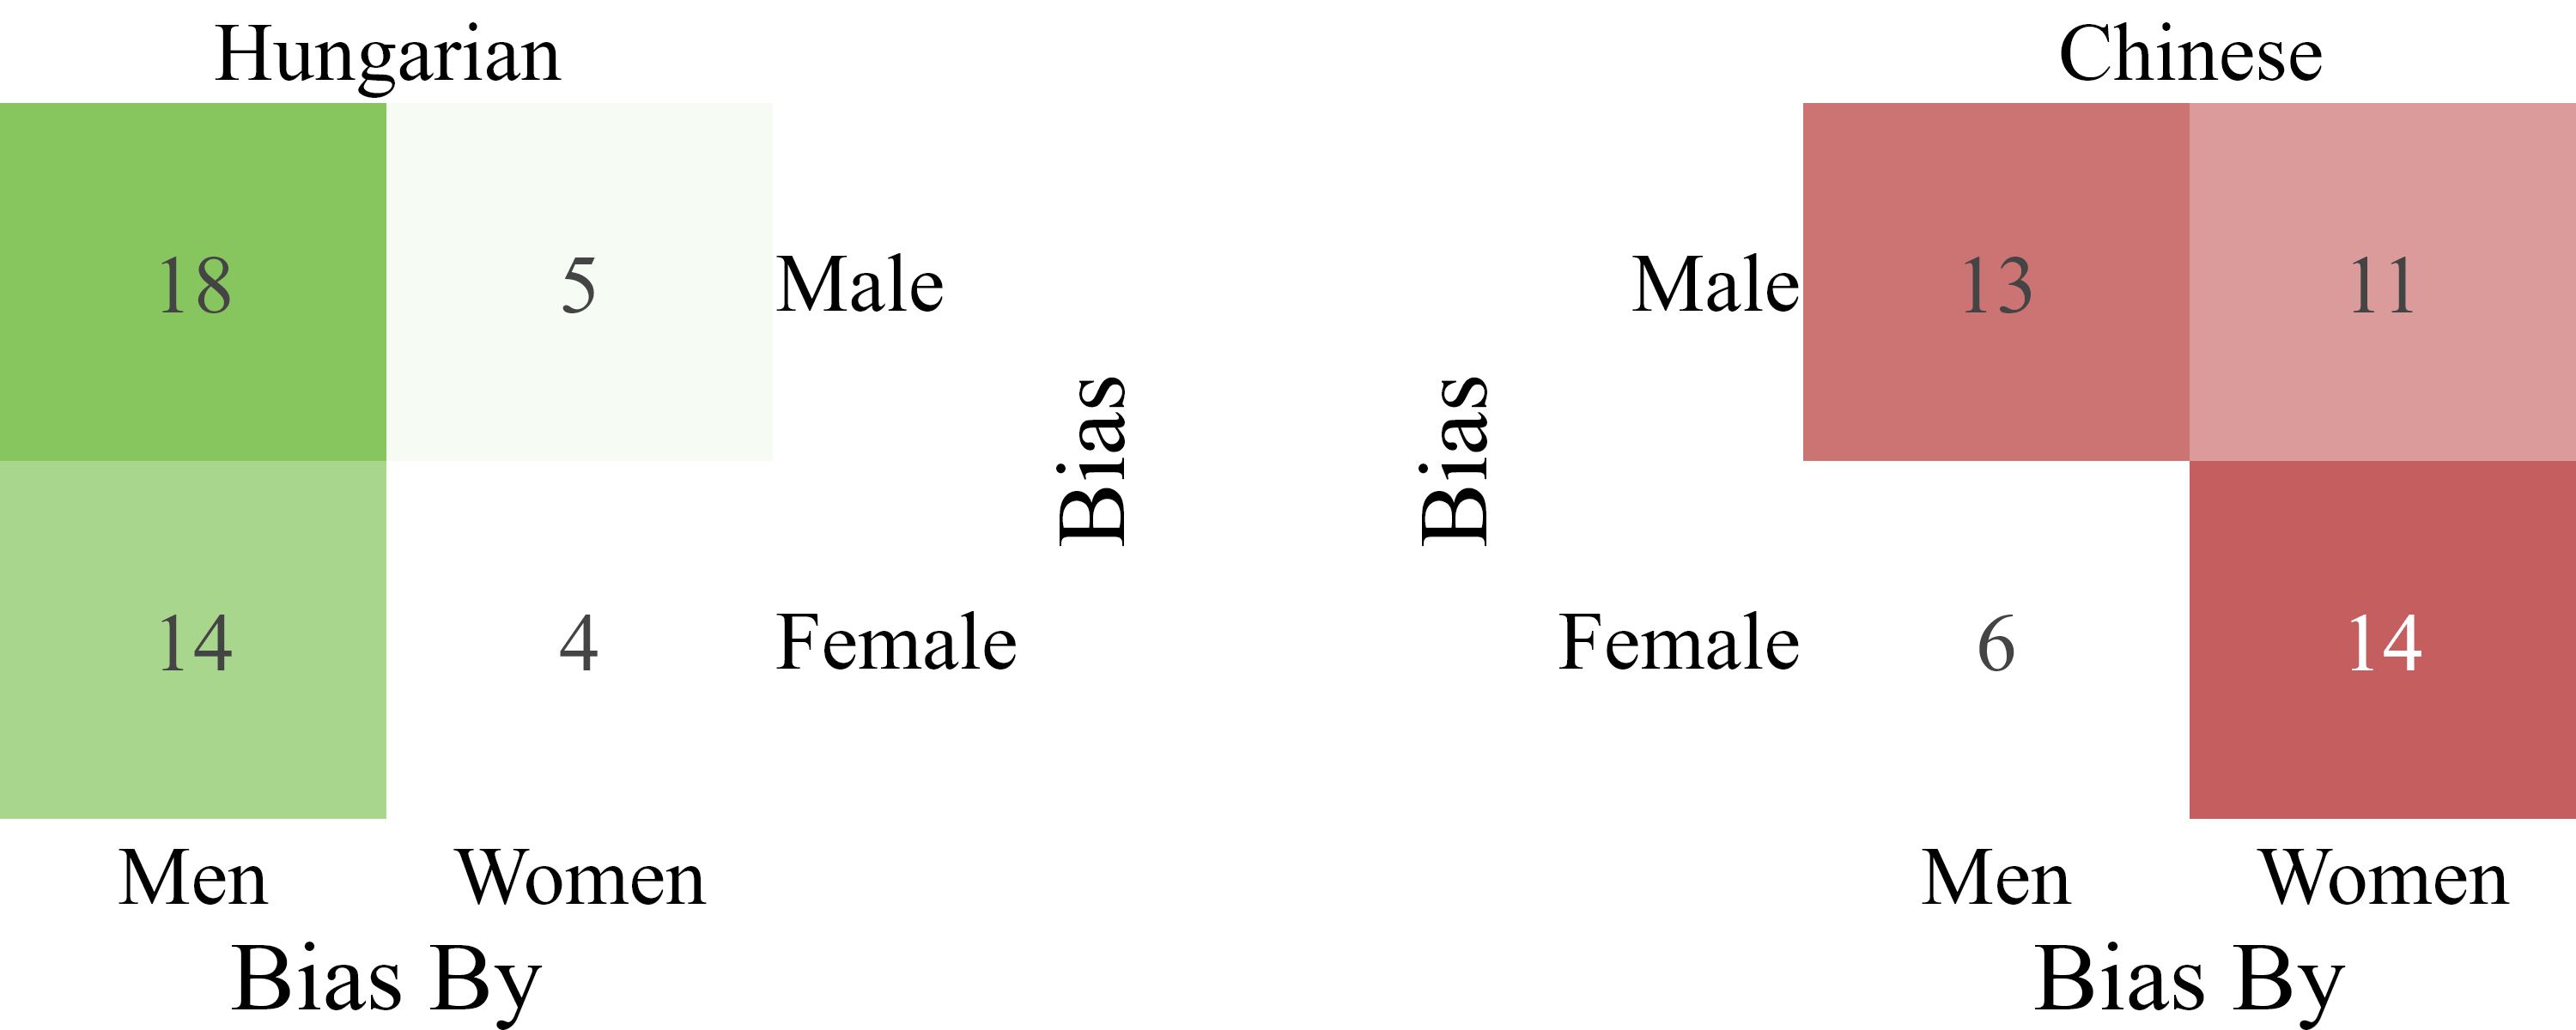
\includegraphics[width=\linewidth]{../confusion_matrices}
  \caption{Confusion matrix of the Hungarian and Chinese ratings, showing the differences in the ratings of male and female participants.}  
  \label{fig:confusion_matrices}
\end{figure}

\subsection{Gender bias by language users' gender}

An interesting divergence arose when comparing the two datasets and the differences between the ratings by gender. While in Hungarian, biases -- both male and female -- were stronger in the ratings of men, in Chinese women rated with a stronger bias on average, especially regarding female biases. You can compare the contrast in Figure \ref{fig:confusion_matrices}.


\begin{figure*}[!ht]
  \centering
  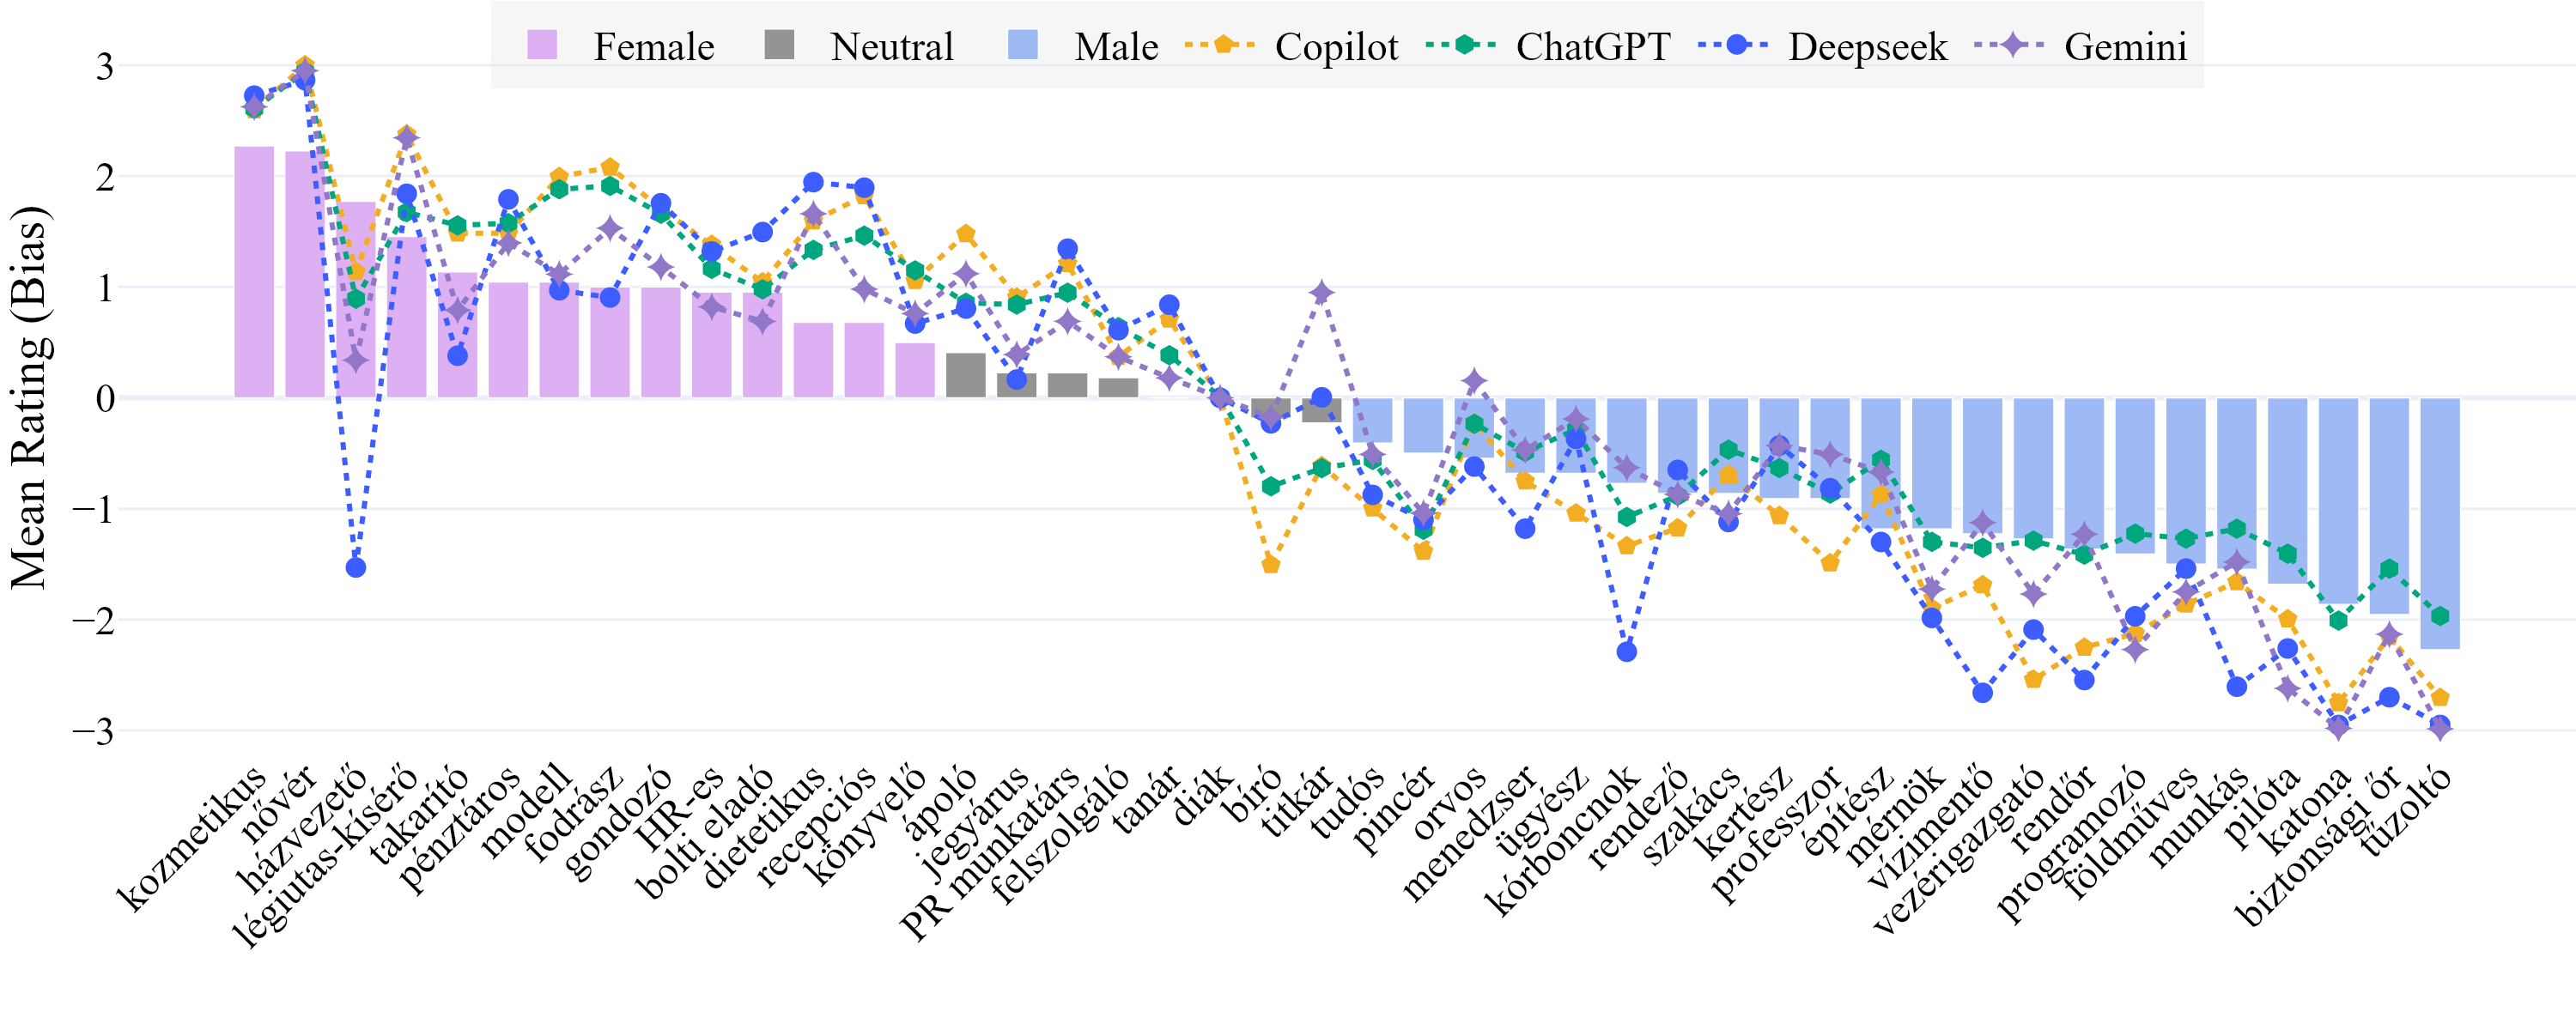
\includegraphics[width=\linewidth]{../occupations_hu_with_ai}
  \caption{AI ratings for Hungarian occupations \href{https://htmlpreview.github.io/?https://github.com/partigabor/occupational-bias/blob/main/occupations_hu_with_ai.html}{--- explore the interactive plot}.}
  \label{fig:occupations_hu_with_ai}
\end{figure*}

\begin{figure*}[tbp]
  \centering
  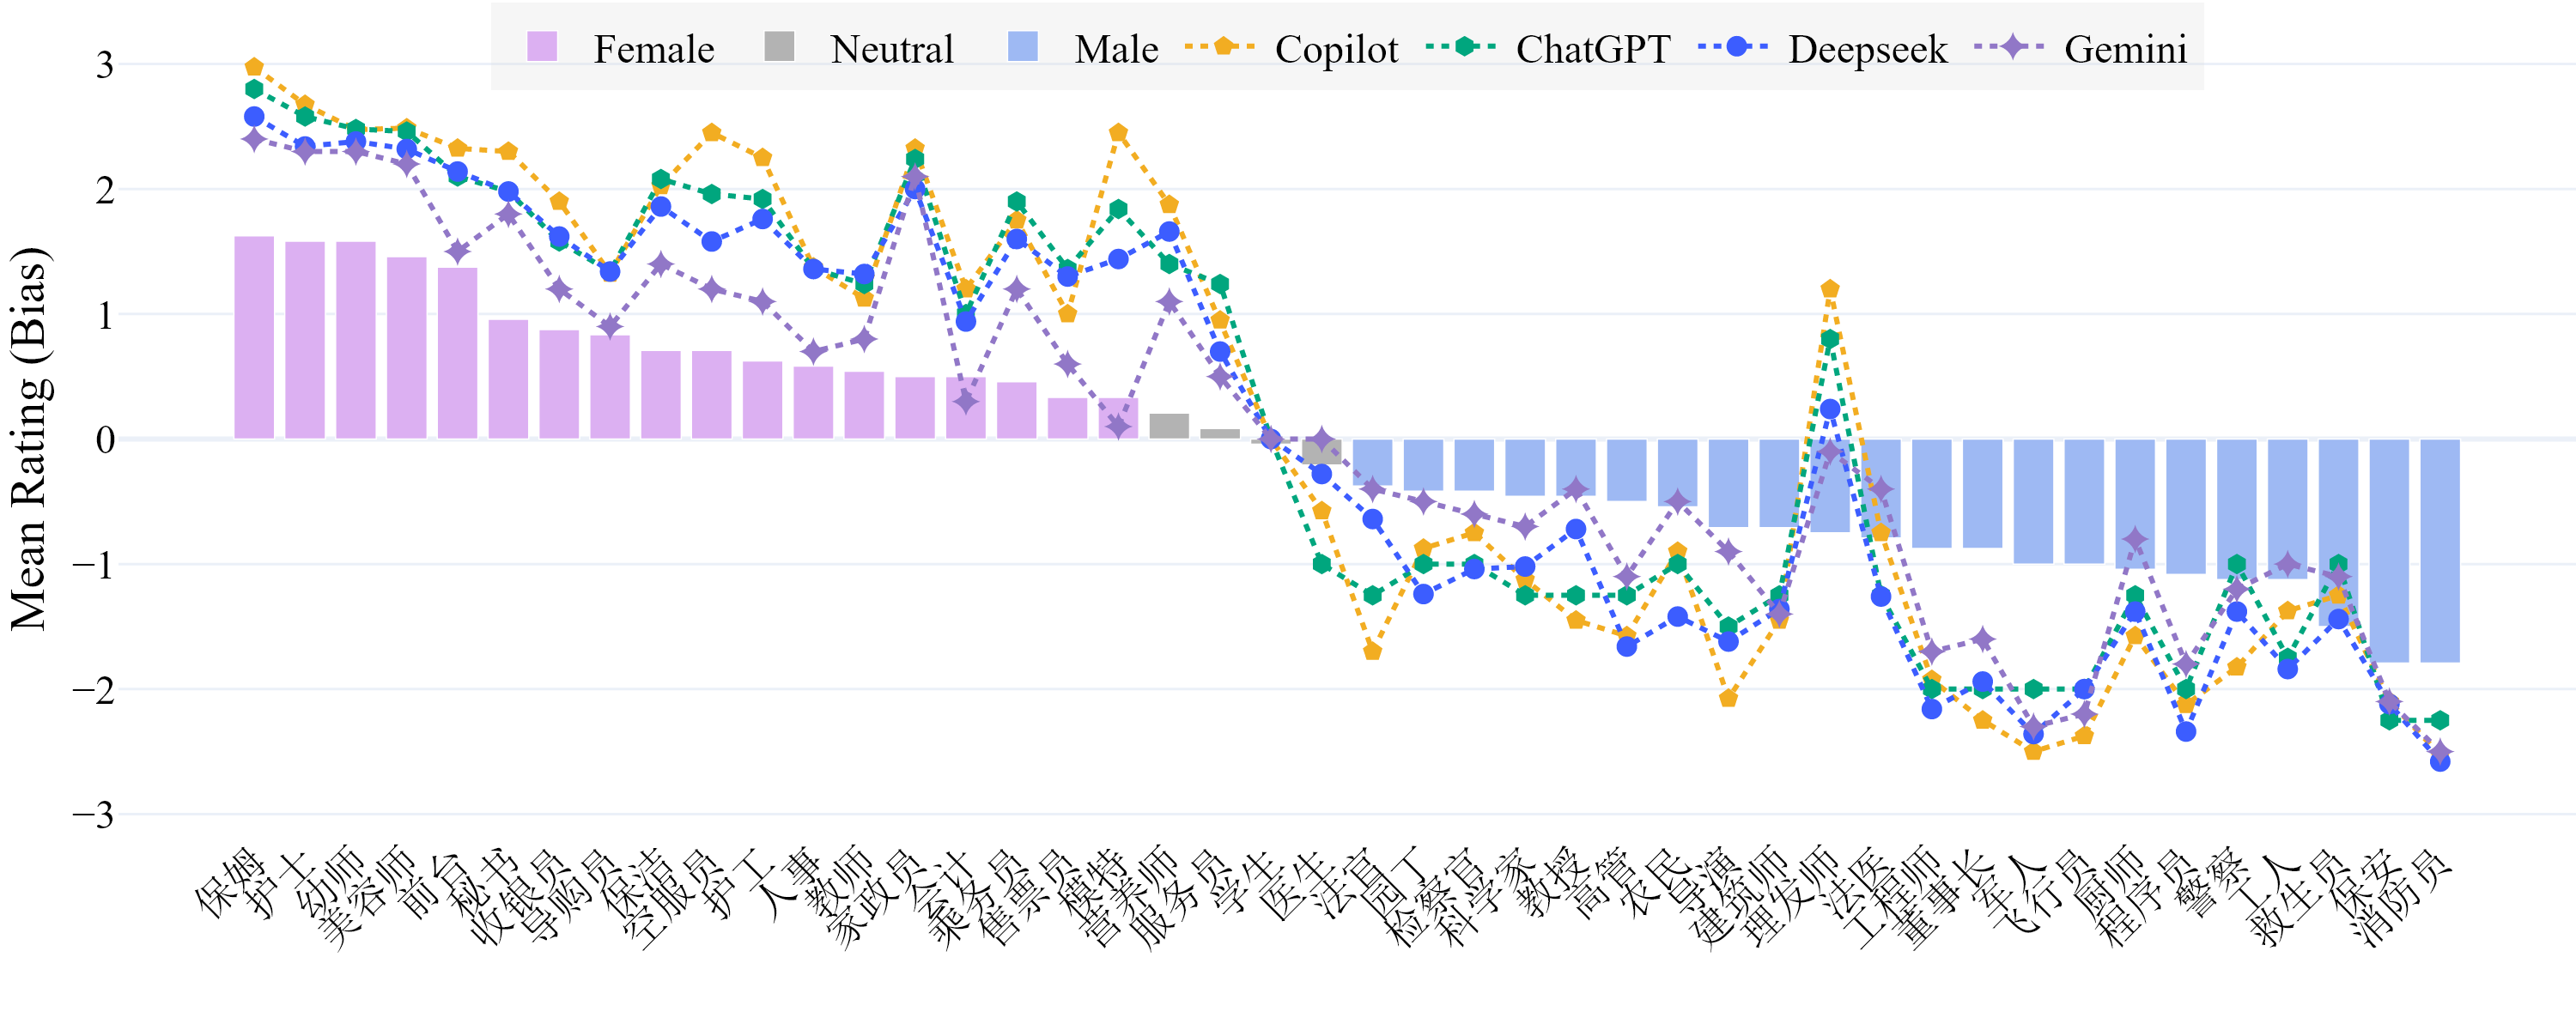
\includegraphics[width=\linewidth]{../occupations_zh_with_ai}
  \caption{AI ratings for Chinese occupations \href{https://htmlpreview.github.io/?https://github.com/partigabor/occupational-bias/blob/main/occupations_zh_with_ai.html}{--- explore the interactive plot}.}
  \label{fig:occupations_zh_with_ai}
\end{figure*}

\section{Comparing the human ratings with AI-generated ratings}

\hl{Gabor is still working on this part...}

Now, we were also curious how the human ratings compare to the ratings of Large Language Models (LLMs) used in popular AI agents, and so we basically repeated the same experiment using AI instead of human raters. We prompted Copilot (+Think Deeper), ChatGPT (+Reason), Gemini (2.5 Flash), and Deepseek (Deepthink R1) to elicit a rating on the same job titles in both languages, using the same scale as the human raters. The instructions were in Hungarian and in Chinese, respectively, with a pretext: ``You are participating in an experiment and your answers will help our research.''. We asked the AI agents 10 separate times, and took the mean as a baseline for the results for each job title. The mean AI ratings were then superimposed on the human raters' plots to allow for a convenient comparison, you can see these in Figures \ref{fig:occupations_hu_with_ai} and \ref{fig:occupations_zh_with_ai}.

The rationale behind this was to simulate how the general public and non-experts would turn to AI to do the job of human raters, and to show that these practices can be highly problematic, as the biases encoded in the LLMs are expected to be even stronger than those of the human raters. \hl{Mention real studies on this and cite}. We think that the results perfectly illustrate the dangers of using AI agents instead of human raters, and only perpetuate social biases.



% ## **4. Discussion (Approx. 1 page)**

% This is where you interpret your results and highlight the importance of your study.

% * **Summary of Findings**: Briefly restate your main findings.
% * **Gender Bias in Ungendered Languages**: Discuss the key takeaway: the absence of grammatical gender does not prevent strong gender stereotypes from being encoded in language and cognition. The bias is likely rooted in societal structures, cultural norms, and extralinguistic context, which are then reflected in word associations.
% * **Cultural Specificity**: Use your cross-linguistic findings to argue for the cultural specificity of some stereotypes. The "hairdresser" example is your strongest evidence here. You can speculate on the cultural reasons for this difference.
% * **The Role of Participant Gender**: Discuss why male and female participants might rate occupations differently. This could relate to personal experience, societal expectations, or in-group/out-group perceptions.
% * **Implications and Future Directions**:
%     * What are the real-world implications of these biases (e.g., in career counseling, job advertisements, AI applications)?
%     * Your comparison with LLMs is highly relevant here. It shows that these societal biases are being learned and potentially amplified by AI systems.
%     * Suggest future research: expanding the list of occupations, including more languages, or using different methodologies (e.g., implicit association tests).
% * **Limitations**: Briefly acknowledge the limitations of your study (e.g., small sample sizes, the specific set of occupations chosen).



\section{Conclusion}


% (This paper aims to show that gender biases exists on the lexical-semantic level, without any real world context, and also that these biases are -- mostly -- comparable even across two distant societies, and presumably everywhere in the developed world.)


In conclusion, our study provides evidence for occupational gender bias in both Hungarian and Chinese contexts, using data from native speakers. We have demonstrated that gender stereotypes are present in job titles, even if the words themselves are unmarked for gender, and this is due to societal norms and cultural influences, reflecting deep-seated biases.

\dots

For the sake of reproducibility and open science, we have made all the data available... please find all raw data and code in this repository: \href{https://github.com/partigabor/occupational-bias}{https://github.com/partigabor/occupational-bias}.

% Make the text font HUGE

\medskip

\noindent{\Large \hl{ANONYMIZE THE FILES BEFORE SUBMISSION!}}

% %%%%%%%%%%%%%%%%%%%%%%%%%%%%%%%%%%%%%%%%%%%%%%%%%%%%%%%%%%%%%%%%%%%%%%%%%%%%%
% %%%%%%%%%%%%%%%%%%%%%%%%%%%%%%%%%%%%%%%%%%%%%%%%%%%%%%%%%%%%%%%%%%%%%%%%%%%%%
% %%%%%%%%%%%%%%%%%%%%%%%%%%%%%%%%%%%%%%%%%%%%%%%%%%%%%%%%%%%%%%%%%%%%%%%%%%%%%



% \section{Introduction}

% These instructions are for authors submitting papers to *ACL conferences using \LaTeX. They are not self-contained. All authors must follow the general instructions for *ACL proceedings,\footnote{\url{http://acl-org.github.io/ACLPUB/formatting.html}} and this document contains additional instructions for the \LaTeX{} style files.

% The templates include the \LaTeX{} source of this document (\texttt{acl\_latex.tex}),
% the \LaTeX{} style file used to format it (\texttt{acl.sty}),
% an ACL bibliography style (\texttt{acl\_natbib.bst}),
% an example bibliography (\texttt{custom.bib}),
% and the bibliography for the ACL Anthology (\texttt{anthology.bib}).

% \section{Engines}

% To produce a PDF file, pdf\LaTeX{} is strongly recommended (over original \LaTeX{} plus dvips+ps2pdf or dvipdf).
% The style file \texttt{acl.sty} can also be used with
% lua\LaTeX{} and
% Xe\LaTeX{}, which are especially suitable for text in non-Latin scripts.
% The file \texttt{acl\_lualatex.tex} in this repository provides
% an example of how to use \texttt{acl.sty} with either
% lua\LaTeX{} or
% Xe\LaTeX{}.

% \section{Preamble}

% The first line of the file must be
% \begin{quote}
% \begin{verbatim}
% \documentclass[11pt]{article}
% \end{verbatim}
% \end{quote}

% To load the style file in the review version:
% \begin{quote}
% \begin{verbatim}
% \usepackage[review]{acl}
% \end{verbatim}
% \end{quote}
% For the final version, omit the \verb|review| option:
% \begin{quote}
% \begin{verbatim}
% \usepackage{acl}
% \end{verbatim}
% \end{quote}

% To use Times Roman, put the following in the preamble:
% \begin{quote}
% \begin{verbatim}
% \usepackage{times}
% \end{verbatim}
% \end{quote}
% (Alternatives like txfonts or newtx are also acceptable.)

% Please see the \LaTeX{} source of this document for comments on other packages that may be useful.

% Set the title and author using \verb|\title| and \verb|\author|. Within the author list, format multiple authors using \verb|\and| and \verb|\And| and \verb|\AND|; please see the \LaTeX{} source for examples.

% By default, the box containing the title and author names is set to the minimum of 5 cm. If you need more space, include the following in the preamble:
% \begin{quote}
% \begin{verbatim}
% \setlength\titlebox{<dim>}
% \end{verbatim}
% \end{quote}
% where \verb|<dim>| is replaced with a length. Do not set this length smaller than 5 cm.

% \section{Document Body}

% \subsection{Footnotes}

% Footnotes are inserted with the \verb|\footnote| command.\footnote{This is a footnote.}

% \subsection{Tables and figures}

% See Table~\ref{tab:accents} for an example of a table and its caption.
% \textbf{Do not override the default caption sizes.}

% \begin{table}
%   \centering
%   \begin{tabular}{lc}
%     \hline
%     \textbf{Command} & \textbf{Output} \\
%     \hline
%     \verb|{\"a}|     & {\"a}           \\
%     \verb|{\^e}|     & {\^e}           \\
%     \verb|{\`i}|     & {\`i}           \\
%     \verb|{\.I}|     & {\.I}           \\
%     \verb|{\o}|      & {\o}            \\
%     \verb|{\'u}|     & {\'u}           \\
%     \verb|{\aa}|     & {\aa}           \\\hline
%   \end{tabular}
%   \begin{tabular}{lc}
%     \hline
%     \textbf{Command} & \textbf{Output} \\
%     \hline
%     \verb|{\c c}|    & {\c c}          \\
%     \verb|{\u g}|    & {\u g}          \\
%     \verb|{\l}|      & {\l}            \\
%     \verb|{\~n}|     & {\~n}           \\
%     \verb|{\H o}|    & {\H o}          \\
%     \verb|{\v r}|    & {\v r}          \\
%     \verb|{\ss}|     & {\ss}           \\
%     \hline
%   \end{tabular}
%   \caption{Example commands for accented characters, to be used in, \emph{e.g.}, Bib\TeX{} entries.}
%   \label{tab:accents}
% \end{table}

% As much as possible, fonts in figures should conform
% to the document fonts. See Figure~\ref{fig:experiments} for an example of a figure and its caption.

% Using the \verb|graphicx| package graphics files can be included within figure
% environment at an appropriate point within the text.
% The \verb|graphicx| package supports various optional arguments to control the
% appearance of the figure.
% You must include it explicitly in the \LaTeX{} preamble (after the
% \verb|\documentclass| declaration and before \verb|\begin{document}|) using
% \verb|\usepackage{graphicx}|.

% \begin{figure}[t]
%   \includegraphics[width=\columnwidth]{example-image-golden}
%   \caption{A figure with a caption that runs for more than one line.
%     Example image is usually available through the \texttt{mwe} package
%     without even mentioning it in the preamble.}
%   \label{fig:experiments}
% \end{figure}

% \begin{figure*}[t]
%   \includegraphics[width=0.48\linewidth]{example-image-a} \hfill
%   \includegraphics[width=0.48\linewidth]{example-image-b}
%   \caption {A minimal working example to demonstrate how to place
%     two images side-by-side.}
% \end{figure*}

% \subsection{Hyperlinks}

% Users of older versions of \LaTeX{} may encounter the following error during compilation:
% \begin{quote}
% \verb|\pdfendlink| ended up in different nesting level than \verb|\pdfstartlink|.
% \end{quote}
% This happens when pdf\LaTeX{} is used and a citation splits across a page boundary. The best way to fix this is to upgrade \LaTeX{} to 2018-12-01 or later.

% \subsection{Citations}

% \begin{table*}
%   \centering
%   \begin{tabular}{lll}
%     \hline
%     \textbf{Output}           & \textbf{natbib command} & \textbf{ACL only command} \\
%     \hline
%     \citep{Gusfield:97}       & \verb|\citep|           &                           \\
%     \citealp{Gusfield:97}     & \verb|\citealp|         &                           \\
%     \citet{Gusfield:97}       & \verb|\citet|           &                           \\
%     \citeyearpar{Gusfield:97} & \verb|\citeyearpar|     &                           \\
%     \citeposs{Gusfield:97}    &                         & \verb|\citeposs|          \\
%     \hline
%   \end{tabular}
%   \caption{\label{citation-guide}
%     Citation commands supported by the style file.
%     The style is based on the natbib package and supports all natbib citation commands.
%     It also supports commands defined in previous ACL style files for compatibility.
%   }
% \end{table*}

% Table~\ref{citation-guide} shows the syntax supported by the style files.
% We encourage you to use the natbib styles.
% You can use the command \verb|\citet| (cite in text) to get ``author (year)'' citations, like this citation to a paper by \citet{Gusfield:97}.
% You can use the command \verb|\citep| (cite in parentheses) to get ``(author, year)'' citations \citep{Gusfield:97}.
% You can use the command \verb|\citealp| (alternative cite without parentheses) to get ``author, year'' citations, which is useful for using citations within parentheses (e.g. \citealp{Gusfield:97}).

% A possessive citation can be made with the command \verb|\citeposs|.
% This is not a standard natbib command, so it is generally not compatible
% with other style files.

% \subsection{References}

% \nocite{Ando2005,andrew2007scalable,rasooli-tetrault-2015}

% The \LaTeX{} and Bib\TeX{} style files provided roughly follow the American Psychological Association format.
% If your own bib file is named \texttt{custom.bib}, then placing the following before any appendices in your \LaTeX{} file will generate the references section for you:
% \begin{quote}
% \begin{verbatim}
% \bibliography{custom}
% \end{verbatim}
% \end{quote}

% You can obtain the complete ACL Anthology as a Bib\TeX{} file from \url{https://aclweb.org/anthology/anthology.bib.gz}.
% To include both the Anthology and your own .bib file, use the following instead of the above.
% \begin{quote}
% \begin{verbatim}
% \bibliography{anthology,custom}
% \end{verbatim}
% \end{quote}

% Please see Section~\ref{sec:bibtex} for information on preparing Bib\TeX{} files.

% \subsection{Equations}

% An example equation is shown below:
% \begin{equation}
%   \label{eq:example}
%   A = \pi r^2
% \end{equation}

% Labels for equation numbers, sections, subsections, figures and tables
% are all defined with the \verb|\label{label}| command and cross references
% to them are made with the \verb|\ref{label}| command.

% This an example cross-reference to Equation~\ref{eq:example}.

% \subsection{Appendices}

% Use \verb|\appendix| before any appendix section to switch the section numbering over to letters. See Appendix~\ref{sec:appendix} for an example.

% \section{Bib\TeX{} Files}
% \label{sec:bibtex}

% Unicode cannot be used in Bib\TeX{} entries, and some ways of typing special characters can disrupt Bib\TeX's alphabetization. The recommended way of typing special characters is shown in Table~\ref{tab:accents}.

% Please ensure that Bib\TeX{} records contain DOIs or URLs when possible, and for all the ACL materials that you reference.
% Use the \verb|doi| field for DOIs and the \verb|url| field for URLs.
% If a Bib\TeX{} entry has a URL or DOI field, the paper title in the references section will appear as a hyperlink to the paper, using the hyperref \LaTeX{} package.

% \section*{Limitations}

% Since December 2023, a "Limitations" section has been required for all papers submitted to ACL Rolling Review (ARR). This section should be placed at the end of the paper, before the references. The "Limitations" section (along with, optionally, a section for ethical considerations) may be up to one page and will not count toward the final page limit. Note that these files may be used by venues that do not rely on ARR so it is recommended to verify the requirement of a "Limitations" section and other criteria with the venue in question.

% \section*{Acknowledgments}

% This document has been adapted
% by Steven Bethard, Ryan Cotterell and Rui Yan
% from the instructions for earlier ACL and NAACL proceedings, including those for
% ACL 2019 by Douwe Kiela and Ivan Vuli\'{c},
% NAACL 2019 by Stephanie Lukin and Alla Roskovskaya,
% ACL 2018 by Shay Cohen, Kevin Gimpel, and Wei Lu,
% NAACL 2018 by Margaret Mitchell and Stephanie Lukin,
% Bib\TeX{} suggestions for (NA)ACL 2017/2018 from Jason Eisner,
% ACL 2017 by Dan Gildea and Min-Yen Kan,
% NAACL 2017 by Margaret Mitchell,
% ACL 2012 by Maggie Li and Michael White,
% ACL 2010 by Jing-Shin Chang and Philipp Koehn,
% ACL 2008 by Johanna D. Moore, Simone Teufel, James Allan, and Sadaoki Furui,
% ACL 2005 by Hwee Tou Ng and Kemal Oflazer,
% ACL 2002 by Eugene Charniak and Dekang Lin,
% and earlier ACL and EACL formats written by several people, including
% John Chen, Henry S. Thompson and Donald Walker.
% Additional elements were taken from the formatting instructions of the \emph{International Joint Conference on Artificial Intelligence} and the \emph{Conference on Computer Vision and Pattern Recognition}.








% Bibliography entries for the entire Anthology, followed by custom entries
%\bibliography{anthology,custom}
% Custom bibliography entries only
\bibliography{custom}

% \appendix

% \section{Example Appendix}
% \label{sec:appendix}

% This is an appendix.

\end{document}
